%\VignetteEngine{knitr::knitr}
%\VignetteIndexEntry{TrendPVA}
% cd '/media/jay/Hitachi2GB/00NMML/activePapers/IliamnaSealsTrendPVA/package/IliamnaSealsTrendPVA/inst/doc'
% Rscript -e "library(knitr); knit('Iliamna-sample.Rnw')"
% pdflatex Iliamna-sample
\documentclass[]{risa}\usepackage[]{graphicx}\usepackage[]{color}
%% maxwidth is the original width if it is less than linewidth
%% otherwise use linewidth (to make sure the graphics do not exceed the margin)
\makeatletter
\def\maxwidth{ %
  \ifdim\Gin@nat@width>\linewidth
    \linewidth
  \else
    \Gin@nat@width
  \fi
}
\makeatother

\definecolor{fgcolor}{rgb}{0.345, 0.345, 0.345}
\newcommand{\hlnum}[1]{\textcolor[rgb]{0.686,0.059,0.569}{#1}}%
\newcommand{\hlstr}[1]{\textcolor[rgb]{0.192,0.494,0.8}{#1}}%
\newcommand{\hlcom}[1]{\textcolor[rgb]{0.678,0.584,0.686}{\textit{#1}}}%
\newcommand{\hlopt}[1]{\textcolor[rgb]{0,0,0}{#1}}%
\newcommand{\hlstd}[1]{\textcolor[rgb]{0.345,0.345,0.345}{#1}}%
\newcommand{\hlkwa}[1]{\textcolor[rgb]{0.161,0.373,0.58}{\textbf{#1}}}%
\newcommand{\hlkwb}[1]{\textcolor[rgb]{0.69,0.353,0.396}{#1}}%
\newcommand{\hlkwc}[1]{\textcolor[rgb]{0.333,0.667,0.333}{#1}}%
\newcommand{\hlkwd}[1]{\textcolor[rgb]{0.737,0.353,0.396}{\textbf{#1}}}%
\let\hlipl\hlkwb

\usepackage{framed}
\makeatletter
\newenvironment{kframe}{%
 \def\at@end@of@kframe{}%
 \ifinner\ifhmode%
  \def\at@end@of@kframe{\end{minipage}}%
  \begin{minipage}{\columnwidth}%
 \fi\fi%
 \def\FrameCommand##1{\hskip\@totalleftmargin \hskip-\fboxsep
 \colorbox{shadecolor}{##1}\hskip-\fboxsep
     % There is no \\@totalrightmargin, so:
     \hskip-\linewidth \hskip-\@totalleftmargin \hskip\columnwidth}%
 \MakeFramed {\advance\hsize-\width
   \@totalleftmargin\z@ \linewidth\hsize
   \@setminipage}}%
 {\par\unskip\endMakeFramed%
 \at@end@of@kframe}
\makeatother

\definecolor{shadecolor}{rgb}{.97, .97, .97}
\definecolor{messagecolor}{rgb}{0, 0, 0}
\definecolor{warningcolor}{rgb}{1, 0, 1}
\definecolor{errorcolor}{rgb}{1, 0, 0}
\newenvironment{knitrout}{}{} % an empty environment to be redefined in TeX

\usepackage{alltt}

\usepackage[figuresright]{rotating}
\usepackage{graphicx, ams, amsmath, amssymb, natbib, setspace}
\usepackage{float}
\usepackage{multirow}
\usepackage[mathscr]{euscript}

% Shortcut commands %%%%%%%%%%%%%%%%%%%%%%%%%%%%%%%%%%%%%%%%%%%%%%%%%%%%%%%%%%%%
\newcommand{\bx}{\ensuremath{\mathbf{x}}}
\newcommand{\bz}{\ensuremath{\mathbf{z}}}
\newcommand{\bbv}{\ensuremath{\mathbf{b}}}
\newcommand{\bcv}{\ensuremath{\mathbf{c}}}
\newcommand{\bs}{\ensuremath{\mathbf{s}}}
\newcommand{\bu}{\ensuremath{\mathbf{u}}}
\newcommand{\cS}{\ensuremath{\mathcal{S}}}
\newcommand{\bb}{\ensuremath{{\boldsymbol{\beta}}}}
\newcommand{\bg}{\ensuremath{{\boldsymbol{\gamma}}}}
\newcommand{\bt}{\ensuremath{{\boldsymbol{\theta}}}}
\newcommand{\bn}{\ensuremath{{\boldsymbol{\eta}}}}
\newcommand{\la}{\ensuremath{\lambda}}
\newcommand{\tr}{{\intercal}}
\def\bc{\mathbf{c}}
\def\bd{\mathbf{d}}
\def\bldf{\mathbf{f}}
\def\bh{\mathbf{h}}
\def\bm{\mathbf{m}}
\def\bn{\mathbf{n}}
\def\br{\mathbf{r}}
\def\bs{\mathbf{s}}
\def\bu{\mathbf{u}}
\def\bv{\mathbf{v}}
\def\bw{\mathbf{w}}
\def\bx{\mathbf{x}}
\def\by{\mathbf{y}}
\def\bz{\mathbf{z}}
\def\bA{\mathbf{A}}
\def\bD{\mathbf{D}}
\def\bG{\mathbf{G}}
\def\bI{\mathbf{I}}
\def\bM{\mathbf{M}}
\def\bQ{\mathbf{Q}}
\def\bR{\mathbf{R}}
\def\bS{\mathbf{S}}
\def\bV{\mathbf{V}}
\def\bW{\mathbf{W}}
\def\bX{\mathbf{X}}
\def\bY{\mathbf{Y}}
\def\bZ{\mathbf{Z}}
\def\cB{\mathcal{B}}
\def\cF{\mathcal{F}}
\def\cI{\mathcal{I}}
\def\cK{\mathcal{K}}
\def\cU{\mathcal{U}}
\def\balpha{\mbox{\boldmath $\alpha$}}
\def\bbeta{\mbox{\boldmath $\beta$}}
\def\bepsilon{\mbox{\boldmath $\epsilon$}}
\def\bdelta{\mbox{\boldmath $\delta$}}
\def\bgamma{\mbox{\boldmath $\gamma$}}
\def\bldeta{\mbox{\boldmath $\eta$}}
\def\bphi{\mbox{\boldmath $\phi$}}
\def\bkappa{\mbox{\boldmath $\kappa$}}
\def\blambda{\mbox{\boldmath $\lambda$}}
\def\bmu{\mbox{\boldmath $\mu$}}
\def\bnu{\mbox{\boldmath $\nu$}}
\def\btheta{\mbox{\boldmath $\theta$}}
\def\brho{\mbox{\boldmath $\rho$}}
\def\bDelta{\mbox{\boldmath $\Delta$}}
\def\bGamma{\mbox{\boldmath $\Gamma$}}
\def\bLambda{\mbox{\boldmath $\Lambda$}}
\def\bSigma{\mbox{\boldmath $\Sigma$}}
\def\var{\textrm{var}}
\def\cov{\textrm{cov}}
\def\log{\textrm{log}}
\def\median{\textrm{median}}
\def\argmin{\textrm{arg min }}
\def\bzero{\mathbf{0}}
\def\bone{\mathbf{1}}
\def\Poi{\textrm{Poi}}
\def\Unif{\textrm{Unif}}
\def\upp{^{\prime}}

\makeindex
\IfFileExists{upquote.sty}{\usepackage{upquote}}{}
\begin{document}
\setcounter{table}{0}
\renewcommand{\thetable}{\Roman{table}}



\jvol{XX}
\jnum{X}
\pubyear{2018}

\doi{10.1111/j.xxxx-xxxx.xxxx.xxxxx.x}
\copyright{2018 Society for Risk Analysis}
\issnyear{xx}

\title[Abundance, Trend and Population Viability for Harbor Seals]{A Bayesian Analysis of Abundance, Trend \\ and Population Viability for Harbor Seals \\ in Iliamna Lake, Alaska}

\author[Peter L. Boveng]{Peter L. Boveng,$^{1}$\affiliation{Marine Mammal Laboratory, Alaska Fisheries Science Center, National Marine Fisheries Service, National Oceanic and Atmospheric Administration, 7600 Sand Point Way NE, Seattle, WA 98115, peter.boveng@noaa.gov}
%%
Jay M. Ver Hoef$^{1}$, David E. Withrow$^{1}$ and Josh M. London$^{1}$} 

\begin{abstract}
Harbor seals in Iliamna Lake, Alaska, are a small, isolated population, and one of only two freshwater populations of harbor seals in the world, yet little is known about their abundance or risk for extinction. Bayesian hierarchical models were used to estimate abundance and trend of this population. Observational models were developed from aerial survey and harvest data, and they included effects for time-of-year and time-of-day on survey counts. Underlying models of abundance and trend were based on a Leslie matrix model that used prior information on vital rates from the literature. We developed three scenarios for variability in the priors and used them as part of a sensitivity analysis. The models were fitted using Markov chain Monte Carlo methods. The population production rate implied by the vital rate estimates was about 5\% per year, very similar to the average annual harvest rate. After a period of growth in the 1980s, the population appears to be relatively stable at around 400 individuals. A population viability analysis assessing the risk of quasi-extinction, defined as any reduction to 50 animals or below in the next 100 years, ranged from 1\% to 3\%, depending on the prior scenario. Although this is moderately low risk, it does not include genetic or catastrophic environmental events, which may have occurred to the population in the past, so our results should be applied cautiously.
\end{abstract}

\begin{keywords}
quasi-extinction, Leslie matrix, demography, survival, hierarchical model
\end{keywords}

\maketitle

% ------------------------------------------------------------------------------
% ------------------------------------------------------------------------------
% ------------------------------------------------------------------------------
% 															INTRODUCTION
% ------------------------------------------------------------------------------
% ------------------------------------------------------------------------------
% ------------------------------------------------------------------------------

\section{Introduction}
\label{sec:intro}
For the management of a natural population of animals, the goals of analysis often include learning about 1) demographic parameters, 2) the population's relationship to the environment, 3) abundance of the population, 4) trend of the population, and 5) viability of the population. All of these goals may be important when making decisions about a population's risk of extinction, such as a listing decision under the U.S. Endangered Species Act. Often, different data sets and analyses are used for the different goals.  However, information on any component is typically expensive to collect and may not be readily available.  In those cases, in order to make the best decision, it may be possible to develop prior distributions on various components from other literature and expert opinion.  In addition, demography, environment, abundance, trend, and viability are all related, and a single model that borrows information from each component and treats uncertainty globally is preferred \citep{Good:meth:2004}.  Although not the only approach, Bayesian models are attractive in this regard, and have been used successfully in the past as integrated analyses \citep{Good:pred:2002, Wade:Baye:2002, Maun:popu:2004}. In this paper, we develop a Bayesian model for incorporating relatively sparse information on counts, harvests, demography, and environmental factors to improve quantitative understanding of abundance, trend, and population viability for a small population of harbor seals, \emph{Phoca vitulina}, inhabiting a large freshwater lake in Alaska.

Iliamna Lake is located in southwest Alaska, and is drained by the Kvichak River to Bristol Bay. It is Alaska's largest freshwater lake, approximately 121 km long, up to 32 km wide and as deep as 300 m \citep{Ande:bath:1969, Haus:Alle:Rich:Quin:resi:2008}.  The seals in Iliamna Lake have been genetically confirmed as harbor seals and there has been no scientific documentation of any rationale for considering them to be a subspecies other than the eastern North Pacific subspecies (\emph{P. v. richardii})\citep{Burn:Van:With:Hole:Asko:inte:2016}. These are one of just five freshwater seal populations in the world, and one of just two harbor seal populations that persist in freshwater, the other consisting of the subspecies \emph{P. v. mellonae}, in the Lacs des Loups Marins of the Ungava Peninsula, Qu\'{e}bec \citep{Smit:Hobs:Koop:Lavi:dist:1996}. The seals in Iliamna Lake appear to be discrete, although there could potentially be interchange with the saltwater seal population in Bristol Bay via the Kvichak River. Genetic analysis and local understanding of the lake seals' isolation suggest that they are a separate population \citep{Burn:Van:With:Hole:Asko:inte:2016,NMFS:enda:2016}.

Seals are observed in the lake year-round and the peak of births occurs in mid-July \citep{Burn:Van:With:Hole:Asko:inte:2016}. The harbor seals in Iliamna Lake make use of abundant salmon runs \citep{Haus:Alle:Rich:Quin:resi:2008}, at least during the summer, as their main prey. Iliamna Lake typically freezes over for much or all of the winter and provides a unique challenge for year-round persistence. When ice covers the lake, fewer seals are observed and little is known about how seals adjust their behavior in response to the ice cover. During that time, harbor seals in the lake likely make use of near-shore leads, cracks, and spaces under the ice for breathing \citep{Burn:Van:With:Hole:Asko:inte:2016}. In the winter, seals are occasionally observed resting on the ice, and harvest by Alaska Natives usually occurs on the ice in spring, before the ice cover breaks up.   

The conservation and management of harbor seals in Iliamna Lake requires decisions that must be made with limited empirical data on demographic parameters, abundance, trend and population viability. Additionally, the data that are available originated from a variety of research projects and methodologies that were not necessarily designed for our objectives. We used aerial surveys of harbor seals in Iliamna Lake conducted by various agencies and organizations, and harvest information, also collected from a variety of sources. Our Bayesian analysis allows flexible inclusion of data from varied sources and allows us to borrow useful information from other harbor seal studies. This framework not only provides the basis for a population viability analysis but sheds light on this unusual ecological setting for harbor seals. We now summarize some of the literature that either informed our development of priors for the Bayesian model, or expresses our expectations about the results.

We examined two main factors associated with variation in observed seal numbers: time-of-year and time-of-day for aerial surveys.  These factors are generally related to when seals haul out of the water.  From studies of seals in saltwater, there is evidence that seals prefer to haul out near the middle of the day, or shortly thereafter \citep{Bove:Beng:With:Cesa:Simp:Fros:Burn:abun:2003,Simp:With:Cesa:Bove:stab:2003,Math:Pend:decl:2006,Ver:Lond:Bove:fast:2010}. However, many other factors are also important, so the time-of-day effect may be weak and complex with considerable variation \citep{Ver:Fros:baye:2003, Lond:VerH:Jeff:Lanc:Bove:haul:2012}.  Nonpup seals undergo molt each year, generally during the month of August in Alaska. It is well established (see literature listed above) that harbor seals in marine environments spend more time hauled out during molt, so we expected to see similar patterns for the harbor seals of Iliamna Lake, with a peak sometime in early to mid-August. We expected to see an earlier peak for pups, with peak pupping in mid-July. However, pups do not molt in their first summer and will start to spend more time foraging (less time hauled out) as they grow.  In addition, the pups grow rapidly and are difficult to distinguish from adults by mid-August when they wean, so we expected their counts to decrease by the time non-pup counts were peaking.

No formal abundance estimates have been made for the harbor seals in Iliamna Lake.  Anecdotal evidence \citep{Burn:unpu:1978} suggested that there may have been around 300 individuals in the 1960s, and a subsequent drop to about 50 after a series of hard winters.  Aerial surveys commenced in 1984 and have been conducted more frequently in recent years. Because harbor seal counts typically vary greatly from day to day, \citet{Math:Klin:harb:1992} suggested summing the highest counts from each haul-out site from multiple surveys in a short time inverval, yielding an estimate of 137 seals in the lake in 1991. Later surveys indicated greater abundance to near 400 seals, with a maximum single-day count of 357 in 2008 \citep{ABR:wild:2011}. Summing the highest site-wise counts as recommended by \citet{Math:Klin:harb:1992} produced estimates of 367, 368, and 389 seals in 2005, 2007, and 2009, respectively.  All estimates lacked an explicit correction for seals that were missed because they were in the water. In saltwater, \citet{Simp:With:Cesa:Bove:stab:2003} estimated that at least 20\% to 35\% of seals would be in the water, even when correcting to hypothetical ideal conditions (of date, time of day, tide, and weather) for hauling out. Using just date, time of day, and tide information from satellite transmitters affixed to seals in nearby Cook Inlet, Alaska, \citet{Ver:Lond:Bove:fast:2010} found that about 40\% of seals would be hauled out under optimum conditions. Those data lacked information from the molt period because satellite transmitters were attached to hair, which falls off during molt.  In summary, previous estimates based on counts are likely to be low, by perhaps 20\% or more.  Thus, our working hypothesis was that seal abundance was slightly over 400 individuals in 2005 - 2009.

With so little documentation of historical abundance, we could only surmise that the population trend may have encompassed an increase since the 1970s, from a low of around 50 seals to recent numbers of around 400. In addition to using observed changes in abundance to estimate trends, rates of survival and reproduction can be used to infer population trend.  However, even less is known about these demographic parameters than abundance for harbor seals in Iliamna Lake.  In fact, very little is known about demographic parameters of harbor seals along the Pacific Rim.  An exception is a detailed study on survival for various sex and age classes at a nearby saltwater site, Tugidak Island, by \citet{Hast:Smal:Pend:sex:2012}.  Little is known about reproduction as well, though \citet{Pitc:Calk:biol:1979} provided data from females in the greater Gulf of Alaska region. Local residents along the lake perceived recent seal numbers to be relatively constant \cite{Burn:Van:With:Hole:Asko:inte:2016}, so we predicted that new data and analysis would indicate a stable population.

Even a population that has been stable faces certain risks if it is small.  Four main risks for species extinctions were outlined by \citet{Shaf:mini:1981}: genetic effects in small populations, demographic stochasticity, environmental stochasticity, and catastrophic events.  All of these apply to populations of any size, but genetic effects and demographic stochasticity are especially important in small populations \citep{Good:demo:1987}. A general rule of thumb was established by \citet{Fran:evol:1980} that a population size greater than 50 was necessary to avoid greatly increased chances of extinction due to genetic effects (but see \citet{Tayl:Roja:1999} for caveats).  After establishing such thresholds, one goal of population viability analysis is to assess the risk, or probability of crossing such a threshold, often called quasi-extinction \citep{Ginz:Slob:John:Bind:quas:1982}, based on current understanding of a population and the ability to project it into the future.  One-hundred years is a common time frame for assessing extinction risk of animals, which represents about 11 generations for harbor seals \citep{Swar:Reij:Pete:Van:abse:1996}. Based on the relatively small population size, we expected that the harbor seals in Iliamna Lake are at considerable risk for crossing into a realm of critically low population size.  

The goal of this paper was to develop a Bayesian hierarchical model based in part on a population process model that includes stochastic variation in vital rates and harvest of seals. Linked to the process model is an observational model for counts from aerial surveys that includes time-of-day and time-of-year effects, and the proportion of seals that are in the water and unavailable to be counted during surveys.  From this model, we wished to obtain estimates of abundance and trend, and project the population into the future to assess the probability of quasi-extinction for different time horizons up to 100 years.  We also wished to perform sensitivity analyses to better understand our prior assumptions. The practical goal of obtaining these results was to provide information for sound management of the harbor seal population in Iliamna Lake.

% ------------------------------------------------------------------------------
% ------------------------------------------------------------------------------
% ------------------------------------------------------------------------------
%                               DATA
% ------------------------------------------------------------------------------
% ------------------------------------------------------------------------------
% ------------------------------------------------------------------------------

\section{DATA}
We conducted aerial surveys of harbor seals in Iliamna Lake between 2008 and 2013. Surveys were conducted in collaboration with local community participants and researchers at the University of Alaska \citep{Burn:Van:With:Hole:Asko:inte:2016}. Surveys were flown using high-wing, twin-engine aircraft (Aero Commander 680, 690 or de Havilland Twin Otter). Survey altitude was typically 330 m and aircraft speed was typically 120 kts. These abundance surveys were performed several times yearly for most years (Table~\ref{tab:surveys}). Surveys were timed so that one survey was conducted while the lake was mostly frozen (Late March/early April), one during pupping (mid-July), and often several during the August molt, when the greatest numbers of seals typically haul out on shore and are visible to aerial observers. Over the years, a comprehensive list of all known haul-out sites was developed. These sites were searched extensively on each flight. Surveys were flown, weather allowing, in the mid- to late-afternoon, when the number of seals hauled out was expected to be highest. Aircraft flight tracks were recorded by GPS and all seals sighted were digitally photographed using a SLR camera (Nikon D700) with zoom lens (Nikkor 80-400mm). Time, date, latitude, longitude, and altitude were automatically embedded into the image metadata. The observer manually recorded weather and visibility information, though the surveys were typically conducted during good conditions and these variables were not used in our analysis. The total number of seals at each haul-out site was counted from the digital photographs. Pups were determined by their smaller size and close proximity ($<$ 1 body length; either nursing or laying right next) to a larger seal. Pups were no longer recorded beyond about mid-August when many had been weaned. By that date the pups were large enough that they could not reliably be distinguished from yearlings and 2-year-olds, which we lumped into the non-pup age class for our analysis. In 2009, researchers from the Newhalen village provided 10 additional flights in collaboration with our survey project, and similar techniques were used. 




\begin{table} 
\centering
  \caption{Summary of Iliamna Lake aerial surveys conducted by various agencies and researchers from 1984 to 2013}
\label{tab:surveys}
\begin{tabular*}{\columnwidth}{@{}l@{\extracolsep{.2cm}}c@{\extracolsep{.2cm}}r@{\extracolsep{.2cm}}r@{\extracolsep{.2cm}}c@{}}
  \Hline
% latex table generated in R 3.4.3 by xtable 1.8-2 package
% Tue Jan 30 18:03:19 2018
Data Source & Year & First Survey & Last Survey & No. of Surveys \\ 
  \hline
\hline
MK92 & 1984 & 1984-08-06 & 1984-08-06 &   1 \\ 
  MK92 & 1987 & 1987-08-29 & 1987-09-10 &   2 \\ 
  MK92 & 1988 & 1988-07-05 & 1988-07-05 &   1 \\ 
  MK92 & 1991 & 1991-08-23 & 1991-08-27 &   8 \\ 
  ADFG & 1998 & 1998-08-13 & 1998-08-23 &   2 \\ 
  ADFG & 1999 & 1999-08-23 & 1999-08-23 &   1 \\ 
  ADFG & 2003 & 2003-08-07 & 2003-08-07 &   1 \\ 
  ABR/Peb & 2005 & 2005-03-30 & 2005-12-13 &  20 \\ 
  MML & 2005 & 2005-08-11 & 2005-08-11 &   1 \\ 
  ABR/Peb & 2007 & 2007-05-22 & 2007-10-11 &   9 \\ 
  ABR/Peb & 2008 & 2008-08-02 & 2008-08-18 &   7 \\ 
  MML & 2008 & 2008-07-24 & 2008-08-20 &   6 \\ 
  MML & 2009 & 2009-05-09 & 2009-08-22 &   7 \\ 
  Newhalen & 2009 & 2009-06-18 & 2009-09-19 &  10 \\ 
  MML & 2010 & 2010-04-03 & 2010-11-03 &   6 \\ 
  MML & 2011 & 2011-04-14 & 2011-11-08 &   6 \\ 
  MML & 2012 & 2012-04-03 & 2012-08-10 &   3 \\ 
  MML & 2013 & 2013-04-05 & 2013-08-08 &   5 \\ 
  
\Hline
\multicolumn{5}{l}{ADFG: Alaska Department of Fish and Game} \\
\multicolumn{5}{l}{MK92: \citet{Math:Klin:harb:1992}} \\
\multicolumn{5}{l}{Newhalen: Community of Newhalen} \\
\multicolumn{5}{l}{MML: Marine Mammal Laboratory,} \\
\multicolumn{5}{l}{\hspace{1cm}NOAA Alaska Fisheries Science Center} \\
\multicolumn{5}{l}{ABR/Peb: \citet{ABR:wild:2011}}
\end{tabular*}
\end{table}

We also used counts obtained prior to 2008 by other organizations. Between 2005 and 2008, \citet{ABR:wild:2011} conducted a series of aerial surveys for harbor seals in Iliamna Lake. In addition, earlier counts from surveys conducted by Alaska Department of Fish and Game (ADFG) \citep{Smal:harb:2001} and surveys from 1984 to 1991 by \citet{Math:Klin:harb:1992} were incorporated into the analysis to expand the historical reach. Geographic coordinates were provided (or, when not provided, determined based on descriptions or physical maps) for each survey site and these sites were compared and merged with locations identified by us. In some cases, sites in very close geographic proximity were combined into a single site. In these surveys, as well as our own, seals  observed in the shallow water near the haul-out site (typically, within 50 m) were included in the counts. It was rare to observe seals in the water away from haul-out sites, and the very few of those that were seen were not included in the counts. A consistent, collated dataset of all five survey projects served as the basis for our analysis. The data we used are archived with the National Centers for Environmental Information \citep{With:Lond:Yano:Bove:aeri:2014} and available for download. Table~\ref{tab:surveys} summarizes the aerial survey effort across the various agencies and researchers.


\begin{table}
\centering
\caption{Harvest data for various communities (column headings) on or near Iliamna Lake.}
\label{tab:harvest}
\begin{tabular*}{\columnwidth}{@{}l@{\extracolsep{0.07cm}}c@{\extracolsep{0.07cm}}c@{\extracolsep{0.07cm}}c@{\extracolsep{0.07cm}}c@{\extracolsep{0.07cm}}c@{\extracolsep{0.07cm}}c@{}}
  \Hline
  Year & Igiugig & Iliamna & Kokhanok & Levelock & Newhalen & PedroBay \\ 
  \hline
  \hline
  1992$^1$ & 2   &     &  11 & 0 &      & \\ 
  1996$^1$ &     &     &     &   &      & 0 \\  
  2004$^1$ &     & 8.5 &     &   & 17.9 & 0 \\  
  2005$^1$ & 5.4 &     & 4.8 & 0 &      & \\  
  2009$^2$ &     &     &   7 &   &    7$^3$ & \\ 
  2010$^1$ &     &     &   0 &   &    2 & \\  
  2011$^1$ & 4.2 & 2.4 & 6.6 & 0 &  7.9 & 1.3 \\  
  \Hline
  \multicolumn{7}{p{.95\columnwidth}}{Table entries are the estimated number of seals harvested by each community for various years.  Fractions occur due to the estimation method, and due to households sharing seal harvest.} \\
  \multicolumn{7}{l}{$^1$\citet{Burn:Van:With:Hole:Asko:inte:2016}} \\
  \multicolumn{7}{l}{$^2$\citet{Burn:Chyt:Gome:Asko:inte:2011}} \\
  \multicolumn{7}{l}{$^3$Burns, Jennifer, Personal Communication, 29 May 2014}
\end{tabular*}
\end{table}

Seals in Iliamna Lake have cultural and nutritional importance to residents of the region \citep{Burn:Van:With:Hole:Asko:inte:2016} and are harvested by local Alaska Native hunters. Hunting primarily occurs in the late winter and early spring when the lake is still ice-covered. As the ice thins and cracks form, the seals haul out along the cracks and are accessible to hunters. Some hunting may go on during summer, but these animals are taken more opportunistically while the earlier hunt is a directed subsistence activity. The numbers of seals harvested from Iliamna Lake have been estimated by household surveys of hunters in the local communities, conducted by the ADFG Subsistence Division \citep{Fall:Hole:Davi:Krie:Kost:subs:2006,Krie:Hole:Kost:subs:2009,Burn:Van:With:Hole:Asko:inte:2016}. We used harvest estimates for the various years between 1992 and 2011 (Table~\ref{tab:harvest}), that were summarized by \citet{Burn:Van:With:Hole:Asko:inte:2016}. We also used estimates from \citet{Burn:Chyt:Gome:Asko:inte:2011}, which were obtained separately from, but by similar methods to the ADFG studies. We did not use values from 1982--1991 that were reported by \citet{Burn:Van:With:Hole:Asko:inte:2016} because we were less certain about whether some of those harvests were from the Kvichak River, rather than Iliamna Lake. Note that because not all households in each community were surveyed, harvest data were estimated such that the values are not necessarily represented as whole numbers of seals per year. 


% ------------------------------------------------------------------------------
% ------------------------------------------------------------------------------
% ------------------------------------------------------------------------------
%                               MODEL
% ------------------------------------------------------------------------------
% ------------------------------------------------------------------------------
% ------------------------------------------------------------------------------

\section{ABUNDANCE, TREND AND POPULATION VIABILITY}
In this section, we describe the basic model for the data, and priors for the model parameters.  We used Markov chain Monte Carlo (MCMC) methods for fitting the model, \citet[e.g.][]{Gilk:Rich:Spie:intr:1996}, which provide a sample from the posterior distribution of the parameters, such as survival and productivity.  That sample also enables inference on derived quantities such as abundance, trend and population viability.

\subsection{The Model} \label{sec:model}
For surveys in the earlier years when pups were not distinguished from non-pups, we denote the combined counts as $Z_{t,i}$ for the $i$th count in the $t$th year.  Later, when pups were distinguished from non-pups, we denote pup counts as $X_{t,i}$ for the $i$th count in the $t$th year, and non-pup counts as $Y_{t,i}$. Harvest data, as given in  Table~\ref{tab:harvest}, are denoted by $H_{t,m}$ for the $t$th year and the $m$th village. We used the follow observational models for harbor seal counts in Iliamna Lake,
\begin{align} \label{eq:modelSetup}
{[}X_{t,i}|\lambda_{t,i},\eta^2]=&\mathcal{N}(\lambda_{t,i}, \eta^2),\nonumber\\ 
{[}Y_{t,i}|\mu_{t,i},\sigma^2]=& \mathcal{N}(\mu_{t,i}, \sigma^2) \nonumber, \\
{[}Z_{t,i}|\lambda_{t,i},\mu_{t,i},\eta^2,\sigma^2] =& \mathcal{N}(\lambda_{t,i} + \mu_{t,i}, \eta^2 + \sigma^2), \nonumber \\
{[}H_{t,m}|\bnu_m,C_m] =& \mathcal{DU}_m(1/C_m), \nonumber \\
 & H_{t,m} \in \{v_1,\ldots,v_{C_m}\}, 
\end{align}
where $\mathcal{N}(a,b)$ is a Gaussian (normal) distribution with mean $a$ and variance $b$, and $\mathcal{DU}(\cdot)$ is a discrete uniform where $H_{t,m}$ takes one of the values $\bnu_m = (v_1,\ldots,v_{C_m})$ with equal probability $1/C_m$ for $C_m$ different classes.  Here, $C_m$ is the number of different years with observations per village, and we simply allow for a discrete uniform distribution on the observed values for each village.

\begin{table*}
\centering
\caption{Table of model parameters, a short description, and a link to the formula where they are defined}
\label{tab:parms}
\begin{tabular*}{11cm}{@{\extracolsep{.2cm}}rlr}
  \Hline
  Parameter & Description & Formula \\ 
  \hline
  \hline
  $\eta^2$ & observation variance of pups &  (1) \\ 
  $\sigma^2$ & observation variance of non-pups &  (1) \\  
  $\alpha_{d,1}; \alpha_{d,2}$ & pup regression parameters for day-of-year & (2)   \\  
  $\alpha_{h,1}; \alpha_{h,2}$ & pup regression parameters for time-of-day & (2)   \\  
  $\beta_{d,1}; \beta_{d,2}$ & non-pup regression parameters for day-of-year & (2)   \\  
  $\beta_{h,1}; \beta_{h,2}$ & non-pup regression parameters for time-of-day & (2) \\ 
  $\psi$ & expected proportion of seals hauled out during counts & (2) \\
  $P_t$ & annual abundance of pups  & (2),(3),(4)   \\  
  $A_t$ & annual abundance of non-pups & (2),(3),(4)   \\
  $\delta_t$ & annual survival of non-pups & (4) \\
  $\kappa_t$ & annual survival of pups to non-pup class & (4) \\
  $\phi_t$ & annual fecundity of non-pups & (4) \\
  $c_t$ & density dependent fecundity & (4) \\
  $\rho$ & scaling factor for density dependent fecundity & (4) \\
  \Hline
\end{tabular*}
\end{table*}


We built our model hierarchically \citep{Cres:Cald:Clar:VerH:acco:2009}.  We assumed that there is some true underlying population value for pups, $P_t$, and non-pups, $A_t$, for each year $t$. However, some part of the population is in the water, away from the haul-out sites, and unobservable, so we denote the proportion that is observable as $\psi$. The observed values, $P_t$ and $A_t$, are also affected by covariates; in this case day-of-year $d_{t,i}$ and hour-of-day $h_{t,i}$. The expected values of the models in Equations (\ref{eq:modelSetup}) are set up as linear models,
%
\begin{align}  \label{eq:linModels}
	\lambda_{t,i} =& \psi P_t + \alpha_{d,1}d_{t,i} + \alpha_{d,2}d^2_{t,i} + \nonumber \\
		& \alpha_{h,1}h_{t,i} + \alpha_{h,2}h^2_{t,i}, \nonumber \\
	\mu_{t,i} =& \psi A_t + \beta_{d,1}d_{t,i} + \beta_{d,2}d^2_{t,i} + \nonumber \\
		& \beta_{h,1}h_{t,i} + \beta_{h,2}h^2_{t,i}, 
\end{align}
%
with regression parameters $\alpha_{d,1}$, $\alpha_{d,2}$, $\alpha_{h,1}$, and $\alpha_{h,2}$ that control how day-of-year and time-of-day affect pup counts, and $\beta_{d,1}$, $\beta_{d,2}$, $\beta_{h,1}$, and $\beta_{h,2}$, which control how day-of-year and time-of-day affect non-pup counts.  Notice that we could model some interaction between $\alpha_{d,\bullet}$ and $\beta_{d,\bullet}$ because, as pups mature during the summer, they cannot be distinguished from non-pups.  However, we have too little information and data for such estimates, and hence we leave $\alpha_{d,\bullet}$ and $\beta_{d,\bullet}$ as free parameters to capture such interactions.

Note that the construction $\psi P_t$ and $\psi A_t$ leads to a nonidentifiability problem in the model. Any increase in $P_t$ can be counteracted by a decrease in $\psi$ so that the product remains unchanged.  We approached the problem as follows. First, we gave total abundance a lower bound by constraining $P_t + \alpha_{d,1}d_{t,i} + \alpha_{d,2}d^2_{t,i} + \alpha_{h,1}h_{t,i} + \alpha_{h,2}h^2_{t,i}$ to be greater than $\max\{X_{i,t}\}/0.9$ for every $t$, and likewise $A_t + \beta_{d,1}d_{t,i} + \beta_{d,2}d^2_{t,i} + \beta_{h,1}h_{t,i} + \beta_{h,2}h^2_{t,i}$ to be greater than $\max\{Y_{i,t}\}/0.9$ for every $t$, or their sum to be greater than $\max\{Z_{i,t}\}/0.9$, depending on how the data were collected in year $t$.   Our justification for such a constraint follows from \citet{Simp:With:Cesa:Bove:stab:2003}. They found that, under optimal conditions, the expected proportion of seals hauled out of the water was around 0.815, but the maximum that was observed across time was between 0.84 and 0.92 (for two different study areas).  Thus, we used a value of 0.9.  Note that, for consistency with  surveys conducted by others previously, we have included seals seen in shallow water near the haul-out sites as part of the fraction of the population that is 'hauled out'. This differs slightly from the convention used in most studies of marine harbor seals, in which only seals actually hauled out on shore are considered to be hauled out and observable.

The nonidentifiability probem is still unsolved if abundance is uniformly distributed from the lower bound to infinity while $\psi$ is constrained between zero and one.  To solve this, we used an informative beta distribution as a prior for $\psi$. With a proper anchoring of $\psi$, there is some information on the haul-out distribution from the surveys because the counts varied considerably. For example, if we could assume that the maximum number of counted seals reflected that 100\% were hauled out, then a mean haul-out rate could be computed from all other surveys with less than the maximum count. The prior distribution helps anchor this distribution to realistic haul-out values, and we discuss our particular choice in the next section.

We also used a constant $\psi$ rather than a temporally-varying $\psi_t$, for several reasons.  First, the number of surveys per year varied considerably.  Allowing $\psi_t$ to vary yearly would allow abundance to essentially ``track'' the yearly maximum, regardless of the number of surveys in that year.  The haul-out time study of \citet{Simp:With:Cesa:Bove:stab:2003} was based on many time periods, so using the maximum across all years was more appropriate.  Secondly, the issue of nonidentifiability exists for the annual variability of $\psi_t$ as well, which would be confounded with the annual variability of $P_t$ and $A_t$.  While we do believe there is annual variability in $\psi$, because of the confounding we interpret $\psi$ as an average across years and inter-annual variability is captured in the posterior variability of $\psi$.

Finally, note that we also tried formulating $X_{t,i}$, $Y_{t,i}$, and $Z_{t,i}$ in equation (\ref{eq:modelSetup}) using negative binomial distributions, and then formulating Equation (\ref{eq:linModels}) as
\begin{align*}
  \lambda_{t,i} = &P_t \exp(\psi + \alpha_{d,1}d_{t,i} + \alpha_{d,2}d^2_{t,i} + \\
	  &\alpha_{h,1}h_{t,i} + \alpha_{h,2}h^2_{t,i}), \nonumber \\
  \mu_{t,i} = &A_t \exp(\psi + \beta_{d,1}d_{t,i} + \beta_{d,2}d^2_{t,i} + \\ 
	  &\beta_{h,1}h_{t,i} + \beta_{h,2}h^2_{t,i}). 
\end{align*}
However, we found that this multiplicative formulation suffered from over-fitting and further confounding, where the regression coefficients $\alpha_{\bullet,\bullet}$ and $\beta_{\bullet,\bullet}$ would attempt to model the zero counts with unrealistic fits that increased $P_t$ and $A_t$ and decreased $\psi$ in order to obtain the fits.  It seems that having $\psi$ as a multiplicative effect, and $\alpha_{\bullet,\bullet}$ and $\beta_{\bullet,\bullet}$ as additive effects in equation(\ref{eq:linModels}), allows for better identification in the model. Equation (\ref{eq:linModels}) is imperfect in the sense that it is not constrained to be nonnegative, nor are the normal distributions used in equation (\ref{eq:modelSetup}), even though our data are counts. We find this acceptable for the stability in model fitting, and it has no impact on our ability to project into the future based on the Leslie matrix model described next, and in Section~\ref{sec:PVA}.  

We embedded a very simple population model that creates a time series and a relation between the numbers of pups and non-pups.  The model included density dependence (\citet[][p. 511]{Casw:matr:2001}) for fecundity, as this is likely where density dependence occurs for seals, 
%
\begin{align}\label{eq:popmod}
    A_t &= \delta_{t-1}A_{t-1} + \kappa_{t-1} P_{t-1} - H_{t-1},  \nonumber \\
		P_t &= c_{t-1}\phi_{t-1}A_{t-1},
\end{align}
%
where $\delta_{t-1}$ is an autoregressive parameter that, in a population model setting, is survival of non-pups from one year to the next; $\phi_{t-1}$ is fecundity, defined to be the proportion of non-pups that produce pups that survive to next year's survey period in mid-summer; $c_{t-1} = \exp(-\rho N_{t-1}/1000)$ is a density dependent factor for fecundity, scaled by a parameter $\rho$, that shrinks $\phi_{t-1}$ towards zero as $N_{t-1} = A_{t-1} + P_{t-1}$ increases;  $\kappa_{t-1}$ is the proportion of pups that survive from the survey period to become yearlings (and enter the non-pup age class); and $H_{t-1}$ is the number of seals from the total population that were harvested in the previous year.

In Equation (\ref{eq:popmod}), absent the harvest, we have used a very simple two-component Leslie matrix model with density dependence (\citet[][p. 511]{Casw:matr:2001}), $\bn_t = \bM_{t-1}\bn_{t-1}$, where
\begin{equation} \label{eq:LesMatForm}
  \bn_t = \left(\begin{array}{c}
    P_t \\
    A_t \\
  \end{array}\right), \ \
  \bM_t = \left( \begin{array}{ll}
      0 & c_t\phi_t \\
      \kappa_t & \delta_t
  \end{array} \right)
\end{equation}
that matches the age class data that we have, namely, counts for pups and non-pups.  The model is stochastic \citep{Wade:Baye:2002}, (\citet[p. 452]{Casw:matr:2001}) because we allow $\delta_t$, $\phi_t$, and $\kappa_t$ to vary randomly with year $t$.  Early Bayesian approaches to population modeling that included Leslie matrix models include \citet{Raft:Give:Zeh:infe:1995} and \citet{Pool:Raft:infe:2000}. A review of embedding Leslie matrix models in a Bayesian inference framework, including stochastic demographic parameters, is provided by \citet{Gros:Crai:Hutc:Baye:2002} and \citet{Buck:Newm:Fern:Thom:embe:2007}.  Other approaches using stochastic demographic parameters include \citet{Cace:Cace:calc:2013}, who studied effective growth rates when demographic parameters are known, or can be assumed known, with random perturbations (whose distribution is part of the interest).  They show how to obtain a stable population state with the effective growth rate.  Our interest centered more on abundance and trend, and not an estimate or a long-term stable state, which is not very informative with just two age classes in equation~(\ref{eq:LesMatForm}). 

Note that for harbor seal counts, population trends have often been modeled with loglinear models, such as Poisson or negative binomial regression \citep{Ver:Fros:baye:2003,Smal:Pend:Pitc:tren:2003,Math:Pend:decl:2006}, where the trend was a linear or quadratic function of time in the mean of the model. In those regression models, the form of the trend component, and how it behaves near the end of the time sequence, largely determines the trend into the future.  There are advantages to demographic models, even very simple ones, especially for population viability analysis. For example, suppose that the trend in the data is slightly positive.  A regression approach will continue the trend, and a population would never go extinct.  However, a demographic model has such a possibility, even for an overall positive trend, due to the stochastic nature of the parameters, which is a more realistic property of populations.

% ------------------------------------------------------------------------------
%                          Priors
% ------------------------------------------------------------------------------

\subsection{Priors} \label{sec:priors}
A summary of model parameters is given in Table~\ref{tab:parms}. To complete the model, we specified prior distributions on the stochastic components,
%
\begin{align*}
&[\eta] = \textrm{UNIF}(0,30), \\
&[\sigma] = \textrm{UNIF}(0,100), \\
&[\alpha_{d,1}] = [\alpha_{d,2}] = [\alpha_{h,1}] = [\alpha_{h,2}] = \textrm{UNIF}(-\infty,\infty), \\
&[\beta_{d,1}] = [\beta_{d,2}] = [\beta_{h,1}] = [\beta_{h,2}] = \textrm{UNIF}(-\infty,\infty), \\
&[P_1] = [A_1] = \textrm{UNIF}(0,\infty),  \\
&\{[\phi_t]; t= 1,\ldots,29\} = \textrm{i.i.d. UNIF}(0,0.5), \textrm{or} \\
& \hspace{1cm} \textrm{Beta(a,b) for two different scenarios}, \\
&\{[\delta_t]; t= 1,\ldots,29\} = \textrm{i.i.d. UNIF}(0.5,1), \textrm{or} \\
& \hspace{1cm} \textrm{Beta(a,b) for two different scenarios}, \\
&\{[\kappa_t]; t= 1,\ldots,29\} = \textrm{i.i.d. UNIF}(0.5,1), \textrm{or} \\
& \hspace{1cm} \textrm{Beta(a,b) for two different scenarios}, \\
&[\rho] = \textrm{UNIF}(0,1), \\
&[\psi] = \textrm{Beta}(5,5)^{30}
\end{align*}
where i.i.d. means independent and identically distributed. Note that in order to start the population model, we needed initial values for $A_1$ and $P_1$, so each of these was given a flat uniform prior distribution.

Most Bayesian analyses require some discussion of the priors \citep{Good:take:2010}.  We used noninformative priors when we could, such as for $\eta$, $\sigma$, $\alpha_{\cdot,\cdot}$, $\beta_{\cdot,\cdot}$, $P_1$, and $A_1$.  However, our sample sizes were quite small, and the form and shape of the prior distribution had a large effect on the other parameters.  To investigate those effects, and present a sensitivity analysis, we developed three scenarios for the demographic parameters fecundity ($\bphi$), non-pup survival ($\bdelta$), and pup survival ($\bkappa$).  A detailed development of these priors is given in the Appendix, and we give an overview here.  

In Table~\ref{tab:scenarios}, the ``base-priors'' scenario, was developed from demographic parameters of harbor seal survival and fecundity given in \citet{Hast:Smal:Pend:sex:2012} and \citet{Pitc:Calk:biol:1979}, respectively.  Survival estimates for both males and females, at two different stages of development for pups, and ages classes $1-3$ and $>3$, were obtained from \citet{Hast:Smal:Pend:sex:2012}.  Because estimates of pup survival were provided at two different stages, we were able to shift a detailed demographic model based on sex and age at the time of birth, to one based on the time of surveys, and collapse it to just two classes, pups and non-pups.  In doing so, we preserved the stable age distribution and population growth rate of the non-shifted and uncollapsed matrix model, and we derived variance estimates for all parameters.  Then, because $\bphi$, $\bdelta$, and $\bkappa$ were constrained to greater than zero and less than one, we matched moments of the estimates and their variances with a beta distribution to provide a prior distribution that met the required constraints (see Appendix for details).

While the base-priors were derived from the best information that we had on demographic estimates, the associated variances represented sampling error and did not necessarily reflect the variability associated with annual variation in the demographic parameters. Also, the base-priors came from a separate, marine population of seals. The data can inform the posterior distributions of $\phi_t$, $\delta_t$, and $\kappa_t$, but when sample sizes are small there is some danger in making the priors too narrow because then those priors will largely determine the results.  Hence, for the ``wide-priors" scenario, we tripled the standard errors of ``base-priors''.  Also, under base-priors, the expectation for population growth rate was around 4\% annually.  To be neutral on population growth rate, we also adjusted the prior means of $\phi_t$, $\delta_t$, and $\kappa_t$ so that population growth rate was 0.  The details are provided in the Appendix and are summarized in Table~\ref{tab:scenarios}.

For a third scenario, ``uniform-priors,'' we used constrained noninformative priors.  For $\bphi$, it would be very unlikely for fecundity to exceed 50\% of all non-pups, considering some of the non-pups are male and some are too young to produce pups.  It would also be very unlikely for non-pup survival to be less than 50\% given the few studies done on harbor seals in Alaska \citep{Hast:Smal:Pend:sex:2012} and elsewhere \citep{Hark:Heid:comp:1990,Cord:Thom:mark:2014,Mack:Durb:Midd:Thom:baye:2008}, where they were all near 90\%.  We used a similar constraint for survival of pups from age at survey to non-pup status.  Given these constraints, we assumed flat prior distributions (Table~\ref{tab:scenarios}).  Notice that under uniform-priors, the distribution on population growth rate is near -5\% annually. 

Finally, we considered the prior distribution for $\psi$, the expected proportion of seals that are observable.  Research in ocean environments along coastal Alaska showed that haul-out rates averaged from 41 to 50\% \citep{Pitc:McAll:move:1981}, with ranges from 20\% to 80\% along the west coast of North America \citep{Sull:beha:1979,Hube:Jeff:Brow:Delo:Vanb:corr:2001,Simp:With:Cesa:Bove:stab:2003,Ver:Lond:Bove:fast:2010}. Using a prior of Beta(5,5) concentrated most of the prior mass between 0.2 and 0.8.  Additionally, the prior was used multiple times, one for each year $t$, otherwise there was a tendency for $P_t$ and $A_t$ to increase without bound, driving the posterior distribution of $\psi$ towards zero.

\begin{table}
\centering
\caption{Three scenarios for priors on demographic parameters derived from literature values.}
\label{tab:scenarios}
\begin{tabular*}{\columnwidth}{@{}r@{\extracolsep{.25cm}}c@{\extracolsep{.25cm}}r@{\extracolsep{0.25cm}}r@{\extracolsep{.25cm}}r@{\extracolsep{.25cm}}r@{}}
  \Hline
  Scenario & Parameter & Mean & Variance & a & b \\ 
  \hline
  \hline
  base-priors & $\delta$ & 0.891 & 0.000317 & 
    272.63 & 33.52 \\ 
  base-priors & $\phi$ & 0.227 & 0.001075 & 
    36.86 & 125.43 \\ 
  base-priors & $\kappa$ & 0.773 & 0.003300 & 
    40.34 & 11.85 \\ 
  \hline
  wide-piors & $\delta$ & 0.843 & 0.002857 &
    38.25 & 7.14 \\ 
  wide-priors & $\phi$ & 0.215 & 0.009675 &
    3.53 & 12.91 \\ 
  wide-priors & $\kappa$ & 0.731 & 0.029702 &
    4.11 & 1.51 \\ 
  \hline
  uniform-priors & $\delta$ & 0.750 & 0.020833 & { } & { } \\ 
  uniform-priors & $\phi$ & 0.250 & 0.020833 & { } & { } \\ 
  uniform-priors & $\kappa$ & 0.750 & 0.020833 & { } & { } \\
  \Hline
  \multicolumn{6}{p{.95\columnwidth}}{Sampling variation alone (base-priors), variation broadened from consideration of other expected sources of variation (wide-priors), and noninformative variation (uniform-priors). These are described in the text and fully developed in the Appendix. The parameters, non-pup survival ($\delta$), fecundity ($\phi$), and pup survival ($\kappa$) are components of Equation (\ref{eq:popmod}). The columns labeled $a$ and $b$ are the beta distribution parameters, derived using moment matching from the mean and variance in the previous columns (see Appendix for details). The uniform distribution in the uniform-priors extend from 0 to 0.5 for $\phi_t$, and 0.5 to 1 for $\kappa_t$ and $\delta_t$.} \\
\end{tabular*}
\end{table}

% ------------------------------------------------------------------------------
%                          Fitting the Model
% ------------------------------------------------------------------------------

\subsection{Fitting the Model}

The model was fitted with Markov Chain Monte Carlo (MCMC) methods using the Metropolis algorithm \citep{Metr:Rose:Rose:Tell:Tell:equa:1953}, which was custom coded in \texttt{R} \citep{R:Deve:Core:ALan:2016}. We used a burn-in of 50,000 iterations, and then kept each 10th sample from the next 100,000 iterations, yielding 10,000 samples.  From the hierarchical model described in Section~\ref{sec:model} and Section~\ref{sec:priors}, we obtained a sample from the posterior distribution,
%
\[
[\eta, \sigma, \balpha, \bbeta, P_1, A_1, \bphi, \bdelta, \bkappa, \rho, \psi | \bx, \by, \bz, \bd, \bh],
\]
where, from Equation (\ref{eq:modelSetup}), $\bx = \{X_{t,i}\}$, $\by = \{Y_{t,i}\}$, and $\bz = \{Z_{t,i}\}$, and from Equation (\ref{eq:linModels}), $\balpha = (\alpha_{d,1}, \alpha_{d,2}, \alpha_{h,1}, \alpha_{h,2})$, $\bbeta = (\beta_{d,1}, \beta_{d,2}, \beta_{h,1}, \beta_{h,2})$, $\bd = \{d_{t,i}\}$, and $\bh = \{h_{t,i}\}$.  The samples from all posterior distributions were checked for convergence, and no problems were found \citep{Jone:Hara:Caff:Neat:fixe:2006}.

There were missing values.  In particular, we had harvest information for just 6 years.  For the years that were missing harvest data, for each iteration of the MCMC algorithm, we imputed one of the observed values, and this was done by village.  Recall that harvest was modeled as a discrete uniform distribution $\mathcal{DU}_m(1/C_m)$. For example in Iguigig where harvest data were 2, 5.4, and 4.2, all missing years were assigned one of these three values, at random for each year, with probability 1/3.  Then, the total harvest for each year was computed as the sum across the observed and imputed values for all villages. Likewise, there were a few seal counts that were missing hour-of-day values, and so for each iteration of the MCMC algorithm we randomly imputed one of the observed values.  These imputations preserved the variation in the observed data for the missing values without explicitly modeling these variables, which were of no direct interest.

% ------------------------------------------------------------------------------
%                          Trend and Abundance
% ------------------------------------------------------------------------------

\subsection{Trend and Abundance} \label{sec:trend}

Let $P_1^{[k]}$ and $A_1^{[k]}$ be the $k$th MCMC sample of the posterior distribution of the true, initial abundance of pups and non-pups, $P_1$ and $A_1$. Then abundance in the following years is determined by the MCMC sample of the demographic parameters and the observed and imputed harvest values,
\begin{align*}
    A^{[k]}_{t+1} &= \delta^{[k]}_tA^{[k]}_t + \kappa^{[k]}_t P^{[k]}_t - H^{[k]}_t, \\
    P^{[k]}_{t+1} &= c^{[k]}_t\phi^{[k]}_t A^{[k]}_t,
\end{align*}
for $t = 1,\ldots\,29$, where $\delta_t^{[k]}$, $\phi_t^{[k]}$, and $\kappa_t^{[k]}$ are the $k$th MCMC samples for $\delta_t$, $\phi_t$, and $\kappa_t$. The $k$th MCMC sample $c^{[k]}_t$ depends on the $k$th MCMC sample, $\rho^{[k]}$, along with $A_t$ and $P_t$. The $k$th MCMC estimate of total abundance then is $N_t^{[k]} = P_t^{[k]} + A_t^{[k]}$ for any $t$.

We used two methods to estimate trend.  To obtain a global estimate of trend for the model, we pooled all of the leading eigenvalues of $\bM_t^{[k]}$ across both $t$ and $k$. As a second method, we used simple linear regression on the the posterior distribution of the annual abundance estimates \citep{John:Frit:agtr:2014}; that is, we simply regressed abundance on year.  We did this for the last 5, 10, and 15 years. An estimate of trend for the most recent 5 years, taken from the $k$th MCMC sample, was computed as the slope of the regression of $N^{[k]}_t;t=26,\ldots,30$ on the integers $1,\ldots,5$, which we denote as $\tau^{[k]}_5$.  Likewise, an estimate of trend for the most recent 10 years, taken from the $k$th MCMC sample, was computed as the slope of the regression of $N^{[k]}_t;t=21,\ldots,30$ on the integers $1,\ldots,10$, which we denote as $\tau^{[k]}_{10}$; and an estimate of trend for the most recent 15 years, taken from the $k$th MCMC sample, was computed as the slope of the regression of $N^{[k]}_t;t=16,\ldots,30$ on $1,\ldots,15$, which we denote as $\tau^{[k]}_{15}$.

% ------------------------------------------------------------------------------
%                          Population Viability
% ------------------------------------------------------------------------------

\subsection{Population Viability} \label{sec:PVA}

For population viability analysis, we wished to project the population for the next 100 years, \citet[e.g.,][]{Ver:popu:2002}. Consider the MCMC samples of the posterior distributions of $\delta^{[k]}_{t}, \kappa^{[k]}_t, \phi^{[k]}_t; t = 1,\ldots,29; k = 1,\ldots,10000$. For each $t = 30,\ldots,129$, we resampled one year, $t\upp$, independently from $t = 1,\ldots,29$, with replacement, and then set $\delta^{[k]}_{t} = \delta^{[k]}_{t\upp}, \kappa^{[k]}_t = \kappa^{[k]}_{t\upp}, \phi^{[k]}_t = \phi^{[k]}_{t\upp}$ for $t = 30,\ldots,129$ and $k = 1,\ldots,10000$.  We also extended harvest into the future.  Initially, we drew $\tilde{H}_{t,m}^{[k]}$ randomly from $\mathcal{DU}_m(1/C_m)$ for the $m$th village, and then summed them, $\tilde{H}_t^{[k]} = \sum_{m=1}^6 \tilde{H}_{t,m}$ for $t = 30,\ldots,129$ and $k = 1,\ldots,10000$. Based on analyses given in the subsequent sections, it appears that the harbor seal population averaged around 350--400 seals, so we allowed for simulated harvest rates (rather than simulated amounts) by scaling harvest to current abundance: $H_t^{[k]} = (\tilde{H}_t^{[k]}/350)N_t^{[k]}$, where $N_t^{[k]}$ is the current estimate of abundance, as described below.  Thus, as the population increases, more seals would be harvested, and also as the population decreases, fewer seals would be harvested.  This scaling seems natural, and keeps the population from becoming negative due to harvest. 

The simulated population abundance, projected into the future for each $k,t$, is 
\begin{align*}
		A^{[k]}_{t+1} =& \delta^{[k]}_{t}A^{[k]}_t + \kappa^{[k]}_{t} P^{[k]}_t - H^{[k]}_{t}, \\
		P^{[k]}_{t+1} =& c^{[k]}_t\phi^{[k]}_t A^{[k]}_t,
\end{align*}
for $t = 30,\ldots,129$ and $k = 1,\ldots,10000$. For any $t,k$ combination, the simulated total population is $N_t^{[k]} = P_t^{[k]} + A_t^{[k]}$, and note that $c^{[k]}_t$ is constant for $\rho^{[k]}$, but changing with $N_t$.

Because $P_t^{[k,j]}$ and $A_t^{[k,j]}$ are positive, and always greater than $ H_t^{[k,j]}$, the population will never reach 0.  In this case, a threshold needs to be defined that reflects a notion of a critical size, below which the population is very unlikely to avoid extinction.  We chose to illustrate the effects of using thresholds of 10, 50, and 100 individuals. Population viability analysis, then, is concerned with the cases when $N^{[k,j]}_t$ drops below a critical threshold, often called quasi-extinction.  Statistical methods similar to those presented here can be found in \citet{Holm:Sabo:Visc:Vinc:Faga:stat:2007}. In the simulated predictions of population values, the first year that $N^{[k,j]}_t$ falls below such a threshold was recorded, for various thresholds. For each $k$, an indicator that the populations falls below $\xi$ by year $T$ is given by, 
\[
f(T,k,c) = \mathcal{I}\left(\sum_{t=1}^T\mathcal{I}(N^{[k]}_t < \xi) > 0\right),
\]
where $\mathcal{I}(\cdot)$ is the indicator function, which is 1 when its argument is true, and 0 otherwise. Across all simulated populations, the proportion of times that a threshold is crossed, accumulated by year, provides an estimate of the probability of crossing the threshold in the years following 2013.  That is, an estimate of crossing some threshold $\xi$ by time $T$ is,
\begin{equation} \label{eq:probThresh}
  \hat{q}(T,c) = \frac{1}{10,000} \sum_{k=1}^{10,000} f(T,k,\xi).
\end{equation}
Note that other uses of PVA include estimating time to extinction \citep{Tayl:reli:1995}, which we do not consider here.

% ------------------------------------------------------------------------------
% ------------------------------------------------------------------------------
% ------------------------------------------------------------------------------
%                                RESULTS
% ------------------------------------------------------------------------------
% ------------------------------------------------------------------------------
% ------------------------------------------------------------------------------

\section{RESULTS}


We first show posterior distributions for the demographic parameters and covariate effects to confirm that the values are reasonable with respect to our understanding of harbor seal biology. We then turn our attention to derived quantities from the model, such as abundance, trend and population viability analysis.

% ------------------------------------------------------------------------------
%           Distributions of Demographic Parameters
% ------------------------------------------------------------------------------

\subsection{Distributions of Demographic Parameters}

The main drivers of trend and abundance are the demographic parameters, $\delta_t$, $c_t$, $\phi_t$, and $\kappa_t$ (see Table~\ref{tab:parms}). Smoothed posterior densities for each of these quantities are given in Figure~\ref{plot-demparms}. For each parameter, all values across the $t$ years were pooled, so the subscript is dropped when discussing these results. The first column in Fig.~\ref{plot-demparms} contains the results under the base-priors scenario (Table~\ref{tab:scenarios}). Note that there is very little change from the prior distributions to the posteriors, indicating a lack of information in the data compared to the priors.  The average value of the posterior for non-pup annual survival rate ($\delta$; first row, first column) was 0.893, for fecundity ($\phi$; second row, first column of Figure~\ref{plot-demparms}) was 0.232, and for pup survival to non-pup status, $\kappa$, it was 0.778. The posterior distribution of the density dependent scaling factor, $c$ (third row, first column of Figure~\ref{plot-demparms}), depends on the posterior distribution of $\rho$ and various values of $N_t$. We show the posterior distribution of $c$ for $N_t = 300, 600, 1200$, which illustrates how fecundity $c\phi$ declines with increasing values of $N_t$ due to density dependence.



\begin{figure}[b]
\centerline{
  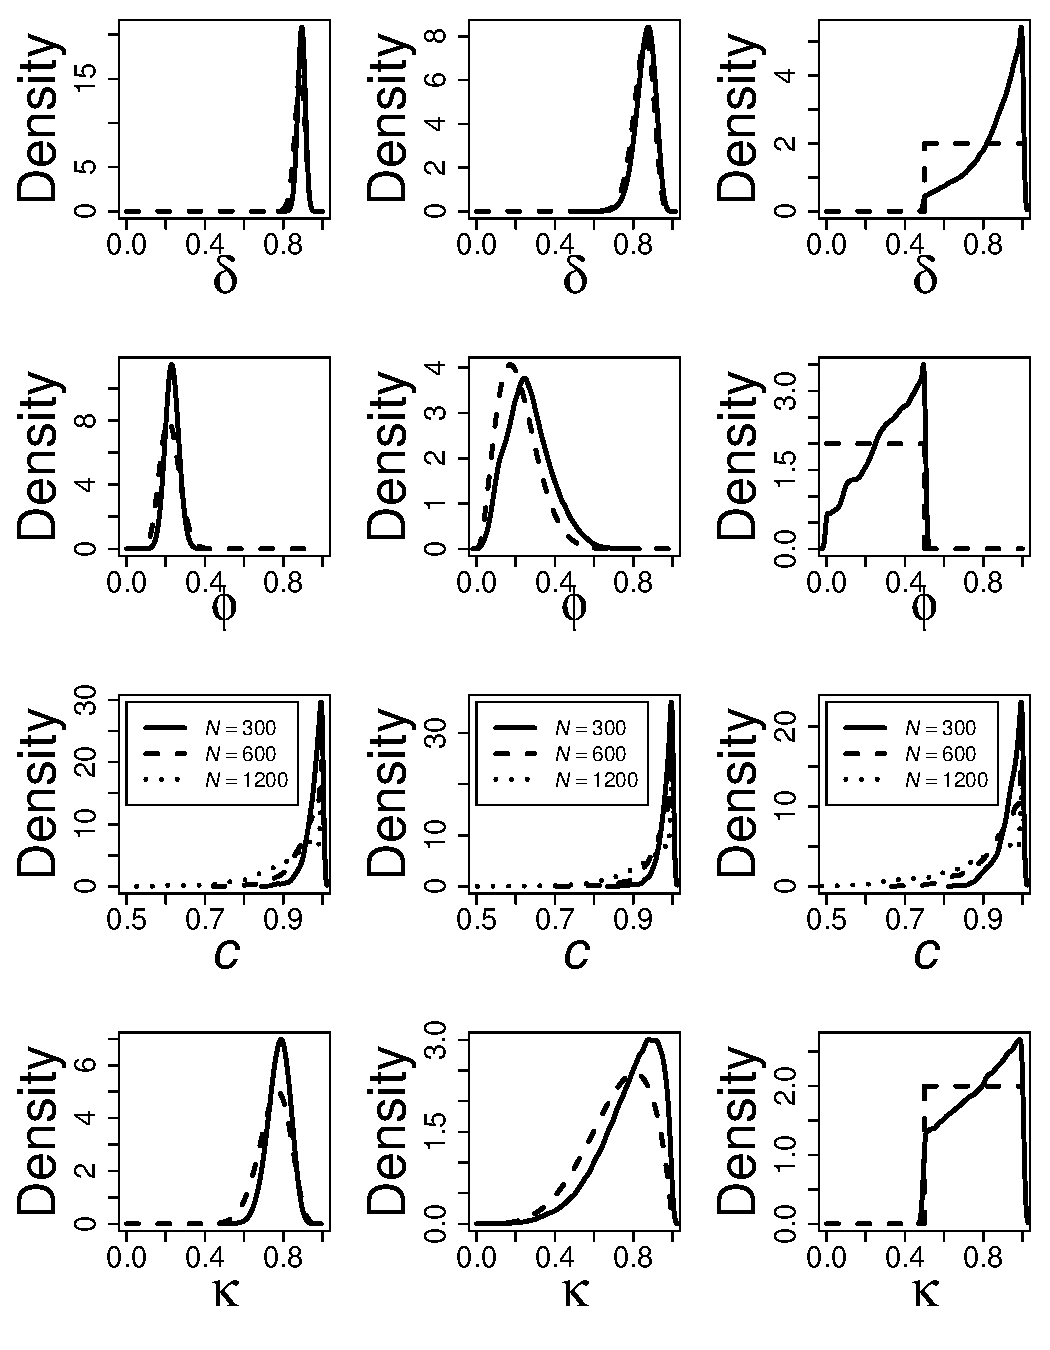
\includegraphics[width=3.25in]{plot-demparms-1.pdf}
}
  \caption{Prior (dashed lines) and posterior (solid lines) densities for adult survival $\delta$, fecundity $\phi$, and pup survival $\kappa$. The posterior densities for density dependence $c$ are also shown for various population sizes $N$. The first column of plots use parameters from the base-priors scenario, and the second and third columns of plots use parameters from wide-priors and uniform-priors, respectively. }  
\label{plot-demparms}       
\end{figure}


The prior distributions were somewhat broader for the wide-priors scenario, and the resulting posteriors diverged more from the priors, shown in the second column of Figure~\ref{plot-demparms}. Here, the average of the posterior values for $\delta$ was 0.861, for $\phi$ was 0.268, and for $\kappa$ was 0.782. The posterior for $c$ for the wide-priors scenario was very similar to that for the base-priors scenario.

The prior distributions were very wide for the uniform-priors scenario, and the resulting posteriors diverged substantially from the priors, as seen from the third column of Figure~\ref{plot-demparms}. The average of the posterior values for $\delta$ was 0.851, for $\phi$ was 0.313, and for $\kappa$ was 0.782. Once again, the posterior distribution of $c$ was similar to both base-priors and wide-priors scenarios.  In all three cases, most of the posterior distribution for $c$ is very near 1.0 for population sizes less than 1000.

% ------------------------------------------------------------------------------
%                 Effects of Date and Time of Day
% ------------------------------------------------------------------------------

\subsection{Effects of Date and Time of Day}


As expected, there was a strong effect of day-of-year on pup counts (Figure~\ref{plot-covariates}A). The mean day-of-year for pup counts was 206 (26 July), and the estimated date of peak pup numbers was 20 July.  Counts as early as day 110 (21 April), and as late as day 301 (29 October), are expected to have around 30 fewer pups than at the peak.  The uncertainty in these temporal patterns is reflected in the variation in the fitted (grey) curves of Figure~\ref{plot-covariates}A. Note that the simple quadratic model may not be fitting very well near the ends of the data, because we would not expect to see any pups at those dates, nor at any dates more than about 3 weeks from the peak. In early April, no pups are born yet, and by late October, they are large enough to be difficult to distinguish from older seals, so these changes reflect both the annual pupping cycle and the decline in observability of older pups. There was a minor peak in the effect of time-of-day on pup counts at about 15:00, which was one hour later than the mean time of the surveys (14:00, Figure~\ref{plot-covariates}B). However, substantial variation among MCMC samples indicated there is little evidence that more pups are expected to be counted at any particular time of day. 

% ------------------------------------------------------------------------------
% 					                  plot-covariates
% ------------------------------------------------------------------------------



\begin{figure}[b]
  \centerline{
    \includegraphics[width=2.75in]{plot-covariates-1.jpeg}
  }
  \caption{The effect of covariates on counts, where each grey line is computed from one MCMC sample of parameters among the 10000 samples from the posterior distribution.  The thick black line is the average value among the 10000 curves. Each curve shows the expected change in counts as a function of the covariate, where all curves pass through the mean covariate value. (A) Day-of-year effect on pup counts, (B) hour-of-day effect on pup counts, (C) day-of-year effect on non-pup counts, and (D) hour-of-day effect on non-pup counts.}
\label{plot-covariates}         
\end{figure}

The peak in expected counts of non-pups occurred later than for pups, on 10 August (Figure~\ref{plot-covariates}C). In comparison to the pups, counts of non-pups decreased more rapidly away from peak counts.  Note that these are expected changes in absolute number, and there are many more non-pups than pups in the population, which can allow for greater increases and declines. The peak count of non-pups was at 13:00 (Figure~\ref{plot-covariates}D), one hour earlier than the mean time of surveys. However, there was considerable variation in the curves and, similar to pup counts, there was only weak evidence for a peak time of day in non-pup counts.

% ------------------------------------------------------------------------------
%                                Abundance
% ------------------------------------------------------------------------------
% ------------------------------------------------------------------------------
% 					                  plot-trendlines
% ------------------------------------------------------------------------------



\begin{figure*}
\centerline{
 \includegraphics[width=5in]{plot-trendlines-1.jpeg}
}
\caption{Series of annual abundance estimates (grey lines) for base-priors (A), wide-priors (C), and uniform-priors (E) from 10000 MCMC samples from the posterior distribution.  The thick black line is the average value over all 10000 samples, the dashed lines form the 2.5\% and 97.5\% point-wise credible intervals, and solid black circles are observed counts. The thin solid line is the average annual abundance estimate times the average $\psi$ value.  Both solids lines are adjusted to optimum covariate conditions. In subfigures B), D), and F), the dashed line is the prior distribution for $\psi$, and the solid line is the posterior distribution, for base-priors, wide-priors, and uniform-priors, respectively.}
\label{plot-trendlines}         
\end{figure*}

\subsection{Abundance} \label{sec:abundance}

For $k = 1,\ldots,10000$ MCMC samples, the abundance estimates $N_t^{[k]}$ for years $t = 1,\ldots,30$ are shown in Figure~\ref{plot-trendlines}A, with priors on the demographic parameters from the base-priors scenario (Table~\ref{tab:scenarios}). For each $t$, the $k$ different averaged values are denoted as $\hat{N}_t$.  Notice the effect of the constraint that $N_t^{[k]}$ must be greater than the maximum observed count in any year, inflated by a factor of 1/0.9. The highest counts in 1998 and 2008 were largely responsible for determining how many seals were missed due to being in the water, from average counts (note that the year ticks are set to 1 January, but surveys generally occurred in summer, and hence the offset in time).  The thin solid line that is fit to the observed data is essentially $\psi \hat{N}_t$, with some correction for covariate effects, reflecting the expected number of seals that are ``observable'' (i.e., at haul-out sites).  The posterior distribution of $\psi$ is shown in Figure~\ref{plot-trendlines}B. Notice that although most of the mass of the prior was between 0.2 and 0.8, the posterior distribution of $\psi$ had most of its mass between 0.35 and 0.5, with a mean of 0.417, indicating that on average slightly more than half of the seals were missed.



Figure~\ref{plot-trendlines}C shows the same information as in Figure~\ref{plot-trendlines}A, but using the wide-priors on the demographic parameters.  Even with the same prior on $\psi$, the greater uncertainty in the prior demographic parameters led to more uncertainty in the abundance, as might be expected (Figure~\ref{plot-trendlines}C). Also note that this greater uncertainty allowed the abundance estimates to ``wrap'' around, to a greater extent, the highest observed values in 1998 and 2008. For the wide-priors scenario, the posterior distribution of $\psi$ is shown in Figure~\ref{plot-trendlines}D, and it appears to be quite similar to that from the base-priors scenario (Figure~\ref{plot-trendlines}B), with a mean of 0.423.

Figure~\ref{plot-trendlines}E shows the same information as given in Figures~\ref{plot-trendlines}A,B, but using the uniform-priors scenario for the demographic parameters.  This scenario had the greatest uncertainty in the prior demographic parameters and led to the greatest uncertainty in the abundance, especially in those years with few or no surveys. For the uniform-priors scenario, the posterior distribution of $\psi$ (Figure~\ref{plot-trendlines}F) again appears to be quite similar to those from the other scenarios, with a mean of 0.434.

% ------------------------------------------------------------------------------
%                                Trend                               
% ------------------------------------------------------------------------------

% 					                  plot-histtrend


\begin{figure}[b]
\centerline{
  \includegraphics[width=3.2in]{plot-histtrend-1.pdf}
}
\caption{Trend summaries from the posterior distribution, computed from the 10000 MCMC samples. The first column is the posterior density of the first eigenvalue of the Leslie matrix, computed on the samples of $\delta$, $\phi$, and $\kappa$ and used in Equation~\ref{eq:LesMatForm}.  The first row is from the base-priors scenario, and rows two and three are from the wide-priors and uniform-priors, respectively.  The second through fourth columns are least-squares linear trends (individuals/year) through the abundance estimates (all of the grey lines in Figure~\ref{plot-trendlines}), for the last 15, 10, and 5 years of abundance estimates, respectively. All posterior densities were smoothed with a kernel density estimator.}
\label{plot-histtrend}         
\end{figure}

\subsection{Trend}

For each MCMC sample $k$, the values $\delta_t^{[k]}$, $c_t^{[k]}$, $\phi_t^{[k]}$, and $\kappa_t^{[k]}$ can be used to form the matrix $\bM_t$ (Equation~\ref{eq:LesMatForm}) for each time period $t$, yielding 290,000 such matrices.  The posterior distributions of the leading eigenvalues from $\bM_t$ are given in the first column of Figure~\ref{plot-histtrend} (matching the situations in Figure~\ref{plot-trendlines}). The leading eigenvalue is the annual factor of increase at the stable age distribution for each Leslie matrix. Despite the fact that the wide-priors scenario had parameters of $\bM_t$ leading to zero growth, and the uniform-priors scenario had parameters of $\bM_t$ leading to negative growth, the posteriors in all three scenarios had means showing positive growth: base-priors scenario  = 1.062, wide-priors scenario = 1.055, and uniform-priors scenario = 1.074.  The base-priors scenario had the least variability, and uniform-priors scenario had the most.

Linear regression estimates of trend were described in Section~\ref{sec:trend}.  In particular, the posterior distribution of the most recent 15 years, using the sample of $\tau^{[k]}_{15}, k = 1,\ldots,10000$, is given in the second column of Figure~\ref{plot-histtrend}.  For the base-priors scenario, there was a posterior probability of 0.5075 of a decreasing trend, indicating little evidence that the population was decreasing over this time period. For the wide-priors scenario, there was a posterior probability of 0.8266, and for uniform-priors, there was a posterior probability of 0.7867, of decreasing trends, neither of which provide strong evidence for a decline.  Nevertheless, these values highlight the difference between the annual factors of population increase computed from the Leslie matrix eigenvalues, which were positive and uncorrected for harvest, and linear trends on the last 15 years of abundance, which were negative and included harvest. 

The posterior distributions of trend for the most recent 10 years, using the sample of $\tau^{[k]}_{10}; k = 1,\ldots,10000$, are given in the third column of Figure~\ref{plot-histtrend}.  For the base-priors scenario, there was a posterior probability of 0.4055 of a decreasing trend, very weak evidence that the population was decreasing over this time period. For the wide-priors scenario, there was a 0.6004 posterior probability, and for uniform-priors a 0.3949 posterior probability, of a decreasing trend, neither of which provides much support for a trend. 

The posterior distributions of trend for the most recent 5 years, using the sample of $\tau^{[k]}_{5}; k = 1,\ldots,10000$, are given in the last column of Figure~\ref{plot-histtrend}.  For the base-priors scenario there was a 0.4961 posterior probability, for wide-priors a 0.584 posterior probability, and for uniform-priors a 0.1383 posterior probability, of a decreasing trend; the latter indicates modest evidence of an increasing trend in the last 5 years.

% ------------------------------------------------------------------------------
%                 subsection  Population Viability Analysis
% ------------------------------------------------------------------------------

\subsection{Population Viability Analysis}

When projecting into the future, as described in Section~\ref{sec:PVA}, the survival and fecundity rates estimated under the base-priors scenario produced little variability (Figure~\ref{plot-PVA}A). Note that for the first 30 years, the lines $N^{[k]}_t; t = 1,\ldots,30$ for $k = 1,\ldots,10000$, are the same as in Figure~\ref{plot-trendlines}A, but plotted on the log scale. The population predictions become more variable when projecting into the future, $N^{[k,j]}_t; t = 31,\ldots,130; k=1,\ldots,10000$. Under this scenario, there was almost no chance that the population would drop below any of the thresholds, $\hat{q}(T,c)$ (Equation~\ref{eq:probThresh}), of 10, 50, or 100 individuals (Figure~\ref{plot-PVA}B). Parameters from the wide-priors scenario produced more variabilty (Figure~\ref{plot-PVA}C). Under this scenario, some of the future population trajectories crossed the various thresholds. The cumulative probability that the population would drop below 100 by year 100 is about 9\%, and there is a 1-2\% chance of dropping below 50 (Figure~\ref{plot-PVA}D). Under the more variable uniform-priors scenario (Figure~\ref{plot-PVA}E), the cumulative probability that the population would drop below 100 is about 5\% within 30 years, and around 15\% by year 100 (Figure~\ref{plot-PVA}F).  There is also about a 4\% chance that the population could drop below 50 by year 100, but still very little chance that the population would drop below 10.



\begin{figure*}
  \centerline{
    \includegraphics[width=5in]{plot-PVA-1.jpeg}
  }
  \caption{Simulated population trajectories (10000 of them) for the next 100 years after year 2013, under the base-priors (A), wide-priors (C), and uniform-priors (E) scenarios. The trajectories for 1984--2013 match those in Figure 3. Each population projection line is mostly transparent, so darker areas have more trend lines through them.   Horizontal lines are thresholds for population sizes of 10, 50, and 100.  Posterior probabilities of quasi-extinction, defined for thresholds of 10, 50, and 100, for various time horizons, are shown in (B), (D), and (F).} 
\label{plot-PVA}        
\end{figure*}

\section{DISCUSSION AND CONCLUSIONS}



\subsection{Demographic Parameters}

\Citet{Hast:Smal:Pend:sex:2012} compared their survival and productivity estimates to other literature on harbor seals in Alaska and elsewhere.  Using their estimates in our base-priors scenario, along with the precision of those estimates, the data did little to move the posterior distributions from the prior distributions (Figure~\ref{plot-demparms}, top row).  However, with our wide-priors and uniform-priors, there was some evidence that both adult survival, $\delta$, and fecundity, $\phi$, were higher than the prior values (Figure~\ref{plot-demparms}, bottom two rows).  This may not be surprising based on traditional knowledge of hunters around Iliamna Lake, who assert that seals in the lake are larger and fatter than their saltwater counterparts \citep{Burn:Van:With:Hole:Asko:inte:2016}. Indeed, in all three scenarios, the posterior distribution of the annual factor of increase (i.e., population growth rate) implied by the Leslie matrix parameters was greater than the prior; (base-priors = 1.062, wide-priors = 1.055, uniform-priors = 1.074).  These growth rates make sense in light of the harvest information (note that the harvest data in the model helped determine them).  On average, Table~\ref{tab:harvest} indicates about 20 seals are harvested per year.  Based on a population of approximately 400, that indicates about 5\% harvest rate, which essentially balances the production rate, consistent with the apparent near-equilibrium in numbers over the past several decades.

\subsection{Effects of Date and Time of Day}

The influence of time-of-day and day-of-year on harbor seal counts in Iliamna Lake mostly matched our expectations from patterns described for marine harbor seals. Despite considerable uncertainty, there was a weak peak just after mid-day for both pups and non-pups around 1400 local time, (Figure~\ref{plot-covariates}B,D), which is very near solar mid-day for this location and exactly the peak time expected from marine harbor seal studies \citep[e.g.,][]{Simp:With:Cesa:Bove:stab:2003}. There was a much stronger relationship to day-of-year. The August peak in Figure~\ref{plot-covariates}C generally matched our expectations, based on the greater amount of time that harbor seals tend to spend ashore when they are most actively molting their pelage.  Pupping generally peaks around mid-June in Alaska \citep{Math:Pend:decl:2006}, but aerial counts are confounded by changes in the absolute numbers of pups, the time that they spend in the water, and the difficulty in distinguishing them from non-pups as they grow during the summer, which generally explains the broad peak in Figure~\ref{plot-covariates}A. A third covariate often modeled for seal counts in marine populations is the effect of tide, which is not present in Iliamna Lake.

\subsection{Abundance and Trends}

The results in Figure~\ref{plot-trendlines} suggest a minimum of around 300 seals occurred in the mid-late 1980s, but there was a large amount of uncertainty, with only a few, relatively low counts obtained during that period (e.g., 77 seals in 1984).  It is likely that the population grew through the 1990s and has stabilized at around 400 individuals.  Using the wide-priors scenario as shown in Figure~\ref{plot-trendlines}C,D, the most recent abundance estimate, in 2013, was 398 with the 95\% credible interval ranging from 326 to 485. The peak abundance estimate in the recent years of increased monitoring occurred in 2008 and was estimated at 460, with the 95\% credible interval ranging from 412 to 536. This corresponds reasonably well with the 389 estimate by \citet{ABR:wild:2011}, which would be expected to be lower because it did not include a correction ($\psi$) for the proportion of seals in the water.

\subsection{Population Viability}

The probability of quasi-extinction in the next 100 years, using 50 as a threshold, was estimated to be around 1\% under wide-priors and 4\% for uniform-priors. We generally disregard the base-priors scenario, as the variances in those priors were developed based on sampling error alone, and not on annual stochastic variation in demographic parameters. In the Introduction, we reported that the concept of extinction risk due to demographic stochasticity is often separated from environmental stochasticity.  However, our analysis includes both because the variation in estimated demographic parameters includes normal environmental variation.  That leaves genetic and catastrophic environmental effects as unmodeled.  A quasi-extinction threshold of 50 may be large enough to avoid genetic effects somewhat, but we acknowledge that populations of long-lived animals that remain at such low levels for very long will likely incur genetic challenges \citep{Fran:rela:1996}.  Finally, it is important to consider catastrophic events. For example, catastrophic population declines have occurred in otariids due to El Ni\~{n}o or unknown causes \citep{Gerb:Hilb:cata:2001}. Our results are based on a span of 30 years, which is a relatively long time for monitoring a marine mammal population. However, a population's risk may depend on rare events that occur less frequently than any observed during the sampling time frame. Based on accounts by local residents, \citet{Burn:unpu:1978} and \citet{Math:Klin:harb:1992} reported that the numbers of seals in Iliamna Lake dropped after extremely severe winters in 1970-71 and 1971-72, to approximately 40 to 50 individuals.  Although the evidence is anecdotal, harbor seals in Iliamna Lake may be subject to such catastrophic events, which increases their risk beyond those that are modeled in this paper.  It is difficult to quantify such catastrophic risk (but see \citet{Ward:Hilb:Towe:Gerb:stat:2007} for a quantitative approach when there are better data), so any management decisions should consider the risk presented in this paper as the minimum risk, and our model could be used to evaluate the effects of hypothetical scenarios for the likelihood of various kinds of catastrophes.

For our data, changes in assumptions (priors) sometimes led to relatively large changes in inference.  For example, the population parameters contained in the scenarios as shown in Figure~\ref{plot-demparms}, led to the different trends (Figure~\ref{plot-histtrend}) and population trajectories (Figure~\ref{plot-PVA}), with differing chances of crossing a quasi-extinction threshold.  As such, these scenarios should be considered a compromise between projections and predictions, in the sense of \citet{Keyf:futu:1972} and \citet[pg. 29]{Casw:matr:2001}.  That is, a prediction is an inference on what \emph{will} happen, and a projection on what \emph{could} happen given a certain set of assumptions.  Here, the data modify the starting assumptions somewhat, but not enough to overwhelm those assumptions.  We have presented several reasonable scenarios through the specification of prior distributions. The results largely match the hypotheses and expectations that we outlined in the Introduction, but the analysis quantified their values and illustrated the uncertainty stemming from the relatively sparse data available for this poorly documented seal population.  This should form a basis for current management decisions, designing future sampling efforts, and a comparison point for future analyses. 

\backmatter

\section*{Acknowledgment}

This paper is dedicated to the memory of Professor Daniel Goodman of Montana State University, who advocated strongly for the use of demography, Bayesian methods, and quantitative risk assessment in conservation decisions. Aerial surveys were authorized under a Marine Mammal Protection Act General Authorization (LOC No. 14590). We thank Paul Conn, Donna Hauser, Kelly Hastings, and Devin Johnson for reviews of early drafts. The findings and conclusions in the paper are those of the authors and do not necessarily represent the views of the reviewers nor the National Marine Fisheries Service, NOAA. Any use of trade, product, or firm names does not imply an endorsement by the US Government.

\section*{Data and Code Accessibility} 

 An \texttt{R} \citep{R:Deve:Core:ALan:2017} package called \texttt{IliamnaSealsTrendPVA} was created that contains all data, code, and analyses. This document was created using \texttt{knitr} \citep{Yihu:impl:2014,Yihu:dyna:2015,Yihu:knit:2016}, and the manuscript combining \LaTeX and \texttt{R} code is also included in the package. The package can be downloaded at 
 \[
 \footnotesize
 \textrm{https://github.com/jayverhoef/IliamnaSealsTrendPVA.git},
 \] 
 with instructions for installing the package.

\bibliographystyle{jmods}
\bibliography{/media/jay/Hitachi2GB/shTex/StatBibTex.bib}



\appendix

\section{:\hspace{2pt} Priors for Demographic Parameters}
\setcounter{table}{0}
\renewcommand{\thetable}{A\Roman{table}}

To develop informative priors, we used the detailed information of sex and age-specific survival obtained from \citet{Hast:Smal:Pend:sex:2012}, and the information on female productivity contained in \citet{Pitc:Calk:biol:1979}, which are given in Table~\ref{tab:demparms}.



The average female fertility rate for all females of age $\ge 3$ was obtained from \citet{Pitc:Calk:biol:1979} in a study of harbor seals in the Gulf of Alaska, the nearest available source for such data. They collected 165 females aged 3+ at various times in the annual cycle between ovulation (early July) and the next pupping-weaning-ovulation season. Among those 165 individuals, 143 had ovulated. \Citet{Pitc:Calk:biol:1979} found that implantation of the embryo took place around early October. There were 132 females in their sample that were collected between the time of implantation and the birth season; 14 of those either failed to become fertilized or lost their embryo or fetus. We estimated the raw birth rate, then, as the ovulation rate (143/165 = 0.867) minus the pregnancy failure rate (14/132 = 0.106), which equals 0.761. Because the females collected for evidence of ovulation and failure of pregnancy were collected at various (unspecified) times in the annual cycle, this raw birth rate accounts incompletely for females that would not have been available to be sampled because of mortality during the interval (i.e., the data are censored). To adjust for this, we applied one-half of the annual mortality rate for the 3+ age class, $(1 - 0.929) / 2 = 0.036$, to the raw birth rate to yield a fecundity rate appropriate for use in a Leslie-type population projection matrix, 0.761 * $(1-0.036) = 0.733$.  The variance was developed assuming indepenent binomial proportions for raw birth rate and pregnancy failure, and used Goodman's result on direct products \citep{Good:on:1960}, assuming again that mortality rate was independent of birth rates and pregnancy failures. 
\begin{table} 
\centering
  \caption{Demographic parameters used to develop informative priors}
\label{tab:demparms}
\begin{tabular*}{\columnwidth}{@{}l@{\extracolsep{\fill}}r@{\extracolsep{\fill}}r@{}}
  \Hline
% latex table generated in R 3.4.3 by xtable 1.8-2 package
% Tue Jan 30 18:03:22 2018
Parameter & Estimate & Standard Error \\ 
  \hline
\hline
Survival Small Male Pups & 0.405 & 0.089 \\ 
  Survival Large Male Pups & 0.717 & 0.088 \\ 
  Survival Male 1-3 & 0.782 & 0.035 \\ 
  Survival Male 3+ & 0.879 & 0.038 \\ 
  Survival Small Female Pups & 0.549 & 0.093 \\ 
  Survival Large Female Pups & 0.820 & 0.069 \\ 
  Survival Female 1-3 & 0.865 & 0.027 \\ 
  Survival Female 3+ & 0.929 & 0.026 \\ 
  Fecundity Female 3+ & 0.733 & 0.041 \\
  \Hline
\end{tabular*}
\end{table}



We began with a full sex- and age-specific Leslie matrix model for harbor seals, then adjusted it for the timing of our surveys, and finally collapsed it to the two classes for which we had information: pups and non-pups.  The full Leslie matrix model, developed from data in \citet{Hast:Smal:Pend:sex:2012} and \citet{Pitc:Calk:biol:1979}, is $\bn_{i+1} = \bM \bn_i$, where $\bM$ is given by
\begin{equation} \label{eq:LesMFull1}
  \left( \begin{smallmatrix} 
 0 & 0 & 0 & 0 & 0 & 0 & 0 & 0.367 \\ 
  0.405 & 0 & 0 & 0 & 0 & 0 & 0 & 0 \\ 
  0 & 0.782 & 0 & 0 & 0 & 0 & 0 & 0 \\ 
  0 & 0 & 0.782 & 0.879 & 0 & 0 & 0 & 0 \\ 
  0 & 0 & 0 & 0 & 0 & 0 & 0 & 0.367 \\ 
  0 & 0 & 0 & 0 & 0.549 & 0 & 0 & 0 \\ 
  0 & 0 & 0 & 0 & 0 & 0.865 & 0 & 0 \\ 
  0 & 0 & 0 & 0 & 0 & 0 & 0.865 & 0.929 \\ 
\end{smallmatrix} \right),
\end{equation}
and $\bn_i$ is
\begin{equation} \label{eq:n1}
  \left(\mbox{\scriptsize$\begin{array}{c}
    n_{\textrm{M,0},i} \\
    n_{\textrm{M,1},i} \\
    n_{\textrm{M,2},i} \\
    n_{\textrm{M,3+},i} \\
    n_{\textrm{F,0},i} \\
    n_{\textrm{F,1},i} \\
    n_{\textrm{F,2},i} \\
    n_{\textrm{F,3+},i} \\
  \end{array} $} \right),
\end{equation}
where $n$ is the number of animals in various sex/age classes, ``M'' indicates male, ``F'' indicates female, ``0'' indates age as birth, ``1'' indicates first birthday, ``2'' indicates second birthday, and ``3+'' indicates birthdays 3 and older. All of the survival values in this model were taken from \citet[][Table 2, part a]{Hast:Smal:Pend:sex:2012}.  We chose these values because they were from a detailed study of well-marked seals, temporally and geographically close to our study in Iliamna Lake. Note that, from genetic considerations, we assumed that the productivity rate was split equally between production of male and female pups, resulting in an expected 0.367 probability of a male pup, and the same probability of a female pup, per female aged 3+.

Our surveys generally occurred around early August.  If not, counts were modeled as being adjusted by a covariate for date as if they were counted in early August.  Hence, there is a misalignment with the demographic parameters in Equation~\ref{eq:LesMFull1} and our observations because seal pups are born prior to most of the aerial surveys.  We corrected for that as follows.  \Citet{Hast:Smal:Pend:sex:2012} gave two survival rates for pups; from the time they are very small, and from the time that they are large.  We take these to be equivalent to the time of birth, and the time of our surveys.  Harbor seal pups grow rapidly, and some time in August it becomes unreliable to distinguish pups from non-pups in aerial surveys, so the survival of large pups aligns very well with our survey period.  For male pups, survival from birth to yearling is reported as 0.405, but survival from a large pup to yearling is 0.717, and hence we take the estimate of survival from small to large pup as 0.405/0.717 = 0.565.  Likewise, the female survival from small to large pup is 0.549/0.82 = 0.67.  We adjusted the productivity values then not for birth, but for the production of pups that survive to the time of surveys.  Hence, females aged 3+ have a 0.367*0.565=0.207 probability of producing a male pup that survives to the survey period, and females aged 3+ have a 0.367*0.67=0.245 probability of producing a female pup that survives to the survey period.  This requires modifying Equation~\ref{eq:LesMFull1} so that $\bM$ is,

\begin{equation} \label{eq:LesMFull2}
   \left( \begin{smallmatrix} 
% latex table generated in R 3.4.3 by xtable 1.8-2 package
% Tue Jan 30 18:03:22 2018
 0 & 0 & 0 & 0 & 0 & 0 & 0 & 0.207 \\ 
  0.717 & 0 & 0 & 0 & 0 & 0 & 0 & 0 \\ 
  0 & 0.782 & 0 & 0 & 0 & 0 & 0 & 0 \\ 
  0 & 0 & 0.782 & 0.879 & 0 & 0 & 0 & 0 \\ 
  0 & 0 & 0 & 0 & 0 & 0 & 0 & 0.245 \\ 
  0 & 0 & 0 & 0 & 0.820 & 0 & 0 & 0 \\ 
  0 & 0 & 0 & 0 & 0 & 0.865 & 0 & 0 \\ 
  0 & 0 & 0 & 0 & 0 & 0 & 0.865 & 0.929 \\ 
  \end{smallmatrix} \right),
\end{equation}
 
There are several characteristics of this population model.  The first (dominant) eigenvalue of the matrix, for both matrices \ref{eq:LesMFull1} and \ref{eq:LesMFull2} is 1.0566, indicating an annual growth rate of 5.66\%. The first eigenvector associated with the dominant eigenvalue for matrix \ref{eq:LesMFull2}, when scaled so that all elements sum to one, is,
\begin{equation}\label{eq:evFull2}
  \bv =  \left( \begin{smallmatrix}
% latex table generated in R 3.4.3 by xtable 1.8-2 package
% Tue Jan 30 18:03:22 2018
 0.081 \\ 
  0.055 \\ 
  0.041 \\ 
  0.179 \\ 
  0.096 \\ 
  0.074 \\ 
  0.061 \\ 
  0.413 \\
  \end{smallmatrix} \right) =
    \left( \mbox{\scriptsize$\begin{array}{c}
    n_{\textrm{M,s},\infty} \\
    n_{\textrm{M,1-2},\infty} \\
    n_{\textrm{M,2-3},\infty} \\
    n_{\textrm{M,3+},\infty} \\
    n_{\textrm{F,s},\infty} \\
    n_{\textrm{F,1-2},\infty} \\
    n_{\textrm{F,2-3},\infty} \\
    n_{\textrm{F,3+},\infty} \\
  \end{array} $} \right)/\textrm{sum}(\bn),
\end{equation}
which is the stable age distribution, shown with $i = \infty$ for the vector, $\bn$, of the number of animals in each sex/age class.  Note that we have changed the notation on $\bn$ to reflect the shift away from birthdays to the time of surveys, indicated by the subscript $s$ on the pup class, and the survey time between birthdays using a dash for other age classes.

Our objective was to collapse the Leslie matrix in \ref{eq:LesMFull2} into two classes. That is, we seek a simplified model
\[
  \left(\begin{array}{c}
    n_{\textrm{pups},i+1} \\
    n_{\textrm{non-pups},i+1} \\
  \end{array}\right) =
    \left( \begin{array}{ll}
      0 & \phi \\
      \kappa & \delta
  \end{array} \right)
    \left(\begin{array}{c}
    n_{\textrm{pups},i} \\
    n_{\textrm{non-pups},i} \\
  \end{array}\right),
\]
where $\phi$ is the probability, among all non-pups alive at one annual survey, of producing a pup that survives to the time of next year's surveys, $\kappa$ is the survival of those pups from the time of aerial surveys to the non-pup class, and $\delta$
is the survival of the non-pups to stay within that class. Assuming the population is at a stable age distribution, from Equation \ref{eq:LesMFull2} and \ref{eq:evFull2}, we used the following weighted averages:


 
\begin{align} \label{eq:delphikap}
  \hat{\delta} = & \frac{ \mathcal{S}_\delta }{\mathcal{D}_\delta}, \nonumber \\
  \hat{\kappa} = & \frac{ \bv_1\bM_{2,1} + \bv_5\bM_{6,5} } { \bv_1 + \bv_5 }, \nonumber \\
  \hat{\phi} = & \frac{\bv_8(\bM_{1,8} + \bM_{5,8})}{\bv_2 + \bv_3 + \bv_4 + \bv_6 + \bv_7 + \bv_8}.
\end{align}
where $\mathcal{S}_\delta = \bv_2\bM_{3,2}+\bv_3\bM_{4,3}+\bv_4\bM_{4,4}+\bv_6\bM_{7,6}+\bv_7\bM_{8,7}+\bv_8\bM_{8,8}$ and $\mathcal{D}_\delta = \bv_2 + \bv_3 + \bv_4 + \bv_6 + \bv_7 + \bv_8$. This yields the matrix
\begin{equation}\label{eq:M2}
  \left( \begin{array}{ll}
      0 & \hat{\phi} \\
      \hat{\kappa} & \hat{\delta}
  \end{array} \right) = 
  \left( \begin{array}{ll}
% latex table generated in R 3.4.3 by xtable 1.8-2 package
% Tue Jan 30 18:03:22 2018
 0.000 & 0.227 \\ 
  0.773 & 0.891 \\ 
  \end{array} \right).
\end{equation}
Notice that, because we used weighted averages of the stable distribution of matrix \ref{eq:LesMFull2}, the eigenvalue of matrix \ref{eq:M2} is 1.0566, which is exactly the same as that for matrix \ref{eq:LesMFull2}, and the stable proportion of pups from matrix \ref{eq:M2} is 0.177, which is exactly the sum of the male and female stable proportions from \ref{eq:evFull2}.

We also developed the variances for the parameters estimated in \ref{eq:M2}.  To do so, we used the delta method \citep{Dorf:anot:1938,Ver:who:2012} twice.  First, consider the following Taylor series approximation for a vector of functions of random variables,
\begin{equation} \label{eq:deltaMeth1}
  \bldf(\bx) \approx \bldf(\bmu) + \bD (\bx - \bmu),
\end{equation}
where,
\[
\bldf(\bx) = \left(\begin{array}{c}
    f_1(\bx) \\
    f_2(\bx) \\
    \vdots \\
    f_\ell(\bx)
  \end{array}\right), \ \
\bldf(\bmu) = \left(\begin{array}{c}
  f_1(\bmu) \\
  f_2(\bmu) \\
  \vdots \\
  f_\ell(\bmu)
\end{array}\right),
\]
and
\[
\bD =  \left(\begin{array}{ccc}
  \frac{\partial f_1(\bx)}{\partial X_1} & \ldots & \frac{\partial f_1(\bx)}{\partial X_m} \\
  \frac{\partial f_2(\bx)}{\partial X_1} & \ldots & \frac{\partial f_2(\bx)}{\partial X_m} \\
  \vdots & \ddots & \vdots \\
  \frac{\partial f_\ell(\bx)}{\partial X_1} & \ldots & \frac{\partial f_\ell(\bx)}{\partial X_m}
\end{array}\right),
\]
and $\bx = (X_1,\ldots,X_m)\upp$ for random variables $X_i$, and $\bmu = E(\bx)$ where the $i$th column of $\bmu$ is $\mu_i$.  Then if $\bSigma$ is the covariance matrix of $\bx$, then
\begin{equation} \label{eq:deltaMeth2}
  \cov(\bldf(\bx)) \approx \bD \bSigma \bD\upp.
\end{equation}
Notice that there are 8 unique entries in \ref{eq:LesMFull2}, but some of them are functions of the quantities in Table~\ref{tab:demparms}. We assume that all variables in Table~\ref{tab:demparms} are independent, so that the covariance matrix is diagonal.  However, using Equation~\ref{eq:deltaMeth2} for the functions of the estimates in Table~\ref{tab:demparms} contained in \ref{eq:LesMFull2} results in the covariance matrix $\bSigma$, which is

\begin{equation} \label{eq:covMentries}
   \left( \begin{smallmatrix}
% latex table generated in R 3.4.3 by xtable 1.8-2 package
% Tue Jan 30 18:03:22 2018
 7.74 & 0 & 0 & 0 & 0 & 0 & 0 & 2.24 \\ 
  0 & 1.23 & 0 & 0 & 0 & 0 & 0 & 0 \\ 
  0 & 0 & 1.44 & 0 & 0 & 0 & 0 & 0 \\ 
  0 & 0 & 0 & 4.76 & 0 & 0 & 0 & 0 \\ 
  0 & 0 & 0 & 0 & 0.73 & 0 & 0 & 1.43 \\ 
  0 & 0 & 0 & 0 & 0 & 0.68 & 0 & 0 \\ 
  0 & 0 & 0 & 0 & 0 & 0 & 2.85 & 0.16 \\ 
  2.24 & 0 & 0 & 0 & 1.43 & 0 & 0.16 & 2.35 \\ 
  \end{smallmatrix} \right) \times 10^{-3},
\end{equation}
among the non-zero entries in \ref{eq:LesMFull2}, where we order them $\bm$ = $(M_{2,1}$, $M_{3,2}$, $M_{4,4}$, $M_{6,5}$, $M_{7,6}$, $M_{8,8}$, $M_{1,8}$, $M_{5,8})$.

Next, notice that $\delta$, $\phi$, and $\kappa$ are functions of the entries in $\bM$, but that function is complicated and nonlinear because some entries occur multiple times in $\bM$, and because of the scaled eigenvector $\bv$. In fact, we can write them showing the dependence on $\bm$ as $\delta(\bm)$, $\phi(\bm)$, and $\kappa(\bm)$, where the exact dependencies are given in Equation~\ref{eq:delphikap}. We need the derivatives of $\delta(\bm)$, $\phi(\bm)$, and $\kappa(\bm)$ with respect to every element of $\bm$.  If we write $f_i(m_j)$, where $m_j$ is the $j$th element of $\bm$ and $f_i(\bm)$ is the $i$th function, which is one of $\delta(\bm)$, $\phi(\bm)$, or $\kappa(\bm)$, then the $i,j$th component of the matrix $\bD$ will be a numeric approximation to the derivative by letting $\bD_{i,j} = (f_i(m_j + h) - f_i(m_j))/h$ for some small value of $h$.  We used $1 \times 10^{-5}$ for both positive and negative values of $h$ for all $i$ and $j$, and tried $1 \times 10^{-4}$ and $1 \times 10^{-6}$ but found there was very little change in $\bD$ for smaller values of $h$.  Then, using Equation~\ref{eq:deltaMeth2} again, with $\bSigma$ as given in \ref{eq:covMentries}, we obtained the following covariance matrix among the estimates of $\delta$, $\phi$, and $\kappa$,

\begin{equation} \label{eq:covmatDelPhiKap}
	\begin{array}{c}
  \hat{\var}\left(\begin{array}{c}
    \hat{\delta} \\
    \hat{\phi} \\
    \hat{\kappa}
  \end{array}\right) = \\
  \left(\begin{smallmatrix}
% latex table generated in R 3.4.3 by xtable 1.8-2 package
% Tue Jan 30 18:03:22 2018
 0.000317 & 0.000171 & -0.000017 \\ 
  0.000171 & 0.001075 & 0.000325 \\ 
  -0.000017 & 0.000325 & 0.003300 \\ 
  \end{smallmatrix}\right).
  \end{array}
\end{equation}


Finally, the prior distributions for these probabilities should be constrained between 0 and 1.  We did this by matching moments with a beta distribution.  A beta distribution, given as
\[
f(x|a,b) = \frac{\Gamma(a + b)}{\Gamma(a)\Gamma(b)}x^{a-1}(1-x)^{b-1},
\]
has 
\begin{align}
E(X) &= \frac{a}{a + b}, \nonumber \\
\var(X) &= \frac{ab}{(a + b + 1)(a + b)^2}. \nonumber
\end{align}
For example, using $\hat{\delta}$ and $\hat{\var}(\hat{\delta})$, we obtained 
\[
a = \frac{\hat{\delta}^2(1-\hat{\delta}) - \hat{\delta}\hat{\var}(\hat{\delta})}
{\hat{\var}(\hat{\delta})},
\]
and then
\[
b = \frac{a(1 - \hat{\delta})}{\hat{\delta}}.
\]
For the estimated value of $\delta$ in (\ref{eq:delphikap}), and its variance in (\ref{eq:covmatDelPhiKap}), we obtained $a =$ 272.63 and $b =$ 33.52. For developing priors, we did not use the estimated covariances among $\hat{\delta}$, $\hat{\phi}$, and $\hat{\kappa}$.


Using this basic framework, we developed three prior scenarios.  ``Base-priors'' used the parameters as estimated above, and moment matching to a beta distribution.  However, notice that the variances in base-priors are estimates for parameters that are assumed fixed, and from a nearby saltwater location.  Our model allows for annual variation in the demographic parameters, and there is little reason to assume that the variance of estimation is related to annual variation. Therefore, it would be prudent to allow the variation to be wider.  We decided to triple the standard errors (nine times the variance of each parameter).  In addition, the base-priors biased the population towards positive growth because the dominant eigenvalue is 1.0566.  In ``wide-priors'', we wanted to be neutral on population growth. Therefore, we wished to scale matrix \ref{eq:M2} so that the eigenvalue was 1.  That is, we wanted to find some $\alpha$ such that
\[
  \left| \bI -
  \lambda\left( \begin{array}{ll}
      0 & \alpha\phi \\
      \alpha\kappa & \alpha\delta
  \end{array} \right) \right| = 0.
\]
Notice that when $\alpha = 1$, $\lambda$ is the eigenvalue of the matrix, so $\alpha = 1/\lambda$ yields an eigenvalue of 1. For the values in \ref{eq:M2}, it is easily determined that $\alpha =$ 0.946 creates the desired matrix. These values, and the variance for wide-priors are given in Table~\ref{tab:scenarios}~, along with the derived $a$ and $b$ parameters for the beta distribution.  As a third scenario, ``uniform-priors'', we used flat uniform priors over the interval 0.5 to 1 for $\delta$ and $\kappa$, and over the interval 0 to 0.5 for $\phi$.  Note that using the mean for each of these parameters yields a dominant eigenvalue of 0.948, biasing the population towards negative growth, but with the widest prior variances.  Our three scenarios are summarized in Table~\ref{tab:scenarios} in the main body of the manuscript.





\end{document}


